\documentclass[
% papersize
a4paper,
%fond size
%12pt,
11pt,
%page print style
twoside,
%oneside,
openright]{book}

%for PSTRicks
\usepackage[pdf]{pstricks}
\usepackage[off]{auto-pst-pdf}

%graphics included tikz & pfg
\usepackage{graphicx}
\usepackage{epsfig,epic,eepic}
\usepackage{psfrag}
\usepackage[USenglish,german]{babel}
\usepackage{color,pstricks}
% To allow me to use letters with accent
\usepackage[latin1]{inputenc}

\usepackage{listings}

% Fonts
%\usepackage{lmodern}
\usepackage[T1]{fontenc}
\usepackage{times}
\usepackage{booktabs}
%\usepackage[scaled]{helvet}
%\usepackage[sc]{mathpazo} % math fonts for Palatino, see
                          % http://www.tug.dk/FontCatalogue/palatino/
%\usepackage{palatino}

% Math packages
\usepackage{amsmath,amssymb,amsfonts,amsthm}
\usepackage{url}
\usepackage[ruled,noline]{algorithm2e}
% More compact lists
\usepackage{paralist}
% Fullpage
\usepackage[in,headings]{fullpage}
% But then adapt spacing
\usepackage{setspace}
\setstretch{1.3}

%for nice tables
\usepackage{multirow}
%\usepackage{booktabs}
\usepackage{ctable}

%for nice item lists
\usepackage{paralist}

%usepackage comment for block comments
\usepackage{comment}

%nice symbols to draw arrow (yes) and -(no)
\usepackage{pifont}
\newcommand{\yes}{\checkmark}
\newcommand{\no}{\textendash}

%sub-picture numbering
\usepackage{subcaption}
%\usepackage{subfigure}

\usepackage[right]{eurosym}


%annotate TODO stuff
\usepackage[colorinlistoftodos, textwidth=4cm, shadow]{todonotes}
\usepackage{lscape}

%pseudocode package
\usepackage{pseudocode}

%to insert some clickable links
\usepackage{hyperref}

\usepackage{fixltx2e}


\definecolor{darkblue}{rgb}{0,0,.5}
\definecolor{black}{rgb}{0,0,0}
\hypersetup{colorlinks=true, breaklinks=true, citecolor=black, linkcolor=black, menucolor=black, urlcolor=black}

% \setlength{\oddsidemargin}{-0.3cm}
% \setlength{\evensidemargin}{-0.3cm}
% \setlength{\textwidth}{16cm}
% \setlength{\topmargin}{-0.8cm}
% \setlength{\textheight}{23.0cm}

% use some common definitions
\newcommand{\pref}[1]{Part~\ref{#1}}
\newcommand{\cref}[1]{Chapter~\ref{#1}}
\newcommand{\sref}[1]{Section~\ref{#1}}
\newcommand{\aref}[1]{Appendix~\ref{#1}}
\newcommand{\fref}[1]{Figure~\ref{#1}}
\newcommand{\tref}[1]{Table~\ref{#1}}
\newcommand{\eref}[1]{(\ref{#1})}

% More convenient sometimes
\newcommand{\ie}{i.\@e.\@ }
\newcommand{\eg}{e.\@g.\@ }

\newcommand{\us}{\,$\mu$s\xspace}

%add empty page macro
\newcommand{\blankpage}{
\newpage
\thispagestyle{empty}
\mbox{}
\newpage
}

% Some math definitions

%\newcommand{\indic}{1\hspace{-2.5mm}{1}}
%\newcommand{\indic}{\boldsymbol{1}}
\newcommand{\indic}[1]{1_{\{#1\}}}
\newcommand{\erfc}{\mathrm{erfc}}
\newcommand{\abs}[1]{\left\lvert #1 \right\rvert}
\newcommand{\lp}[1]{\left( #1 \right)}
\newcommand{\lb}[1]{\left\lbrack #1 \right\rbrack}
\newcommand{\lc}[1]{\left\lbrace #1 \right\rbrace}
\newcommand{\erf}[1]{\mathrm{erf}\lp{#1}}
\newtheorem{definition}{Definition}
\newtheorem{lemma}{Lemma}
\newtheorem{theorem}{Theorem}

\newcommand{\calI}{\mathcal I}
\newcommand{\calN}{\mathcal N}
\newcommand{\calP}{\mathcal P}
\newcommand{\calX}{\mathcal X}
\newcommand{\calC}{\mathcal C}

% Paper specific notation
\def\su{^{(u)}}
\def\s0{^{(0)}}
%
\def\Xr{X^{(r)}}
\def\Xt{X^{(t)}}
%
\def\Ns{N_{\textrm{s}}}
\def\Na{N_{\textrm{a}}}
%
\def\tacq{t_{\textrm{acq}}}
\def\ttx{t_{\textrm{tx}}}
\def\tfail{t_{\textrm{fail}}}
\def\tdrop{t_{\textrm{drop}}}
%
\def\tprop{t_{\textrm{prop}}}
\def\tpreamble{t_{\textrm{preamble}}}
\def\tdata{t_{\textrm{DATA}}}
\def\tack{t_{\textrm{ACK}}}
\def\tsigidle{t_{\textrm{SIGIDLE}}}
\def\tmaxbackoff{t_{\textrm{max backoff}}}
\def\tsendtimer{t_{\textrm{send timer}}}
\def\tidletimer{t_{\textrm{idle timer}}}
\def\tbackoff{t_{\textrm{backoff}}}
%
\def\SD{S_{\textrm{D}}}
\def\SI{S_{\textrm{I}}}
%
\def\Pacq{p_{\textrm{acq}}}
\def\Pfail{p_{\textrm{fail}}}
\def\Pbusy{P_{\textrm{busy}}}
\def\Pmd{P_{\textrm{MD}}}
\def\Pfa{P_{\textrm{FACQ}}}
%
\def\td{t_{\textrm{D}}}
\def\ti{t_{\textrm{I}}}
\def\Np{N_{\textrm{p}}}


\newcommand{\mand} {\mathrm{\;  and \; }}
\newcommand{\mfor} {\mathrm{\;  for \;  }}
\def\Ints{\mathbb{Z}}
\def\P{\mathbb{P}}
\def\E{\mathbb{E}}
\def\be{\begin{equation}}
\def\ee{\end{equation}}
\def\ben{\[}
\def\een{\]}
\def\bearn{\begin{eqnarray*}}
\def\eearn{\end{eqnarray*}}
\def\bear{\begin{eqnarray}}
\def\eear{\end{eqnarray}}
\def\barr{\begin{array}}
\def\earr{\end{array}}
\def\bel{\be \barr{l}}% equation array adjusted left, numbered
\def\eel{\earr\ee}
\def\beln{\ben \barr{l}}% equation array adjusted left, no number
\def\eeln{\earr\een}\def\be{\begin{equation}}
\def\ee{\end{equation}}
\def\ben{\[}
\def\een{\]}
\def\bearn{\begin{eqnarray*}}
\def\eearn{\end{eqnarray*}}
\def\bear{\begin{eqnarray}}
\def\eear{\end{eqnarray}}
\def\barr{\begin{array}}
\def\earr{\end{array}}
\def\bel{\be \barr{l}}% equation array adjusted left, numbered
\def\eel{\earr\ee}
\def\beln{\ben \barr{l}}% equation array adjusted left, no number
\def\eeln{\earr\een}


% Style headings + headers and footers

% Modify header and footers
\usepackage{fancyhdr}
\pagestyle{fancy}
\fancyhf{}
\renewcommand{\chaptermark}[1]{
  \markboth{\thechapter.\ #1}{}
%  \markboth{#1}{}
}
\renewcommand{\sectionmark}[1]{
%  \markboth{\thechapter.\ #1}{}
  \markright{#1}
}

% \fancyhead[LE]{\normalfont\sffamily\thepage}
% \fancyhead[RE]{\normalfont\sffamily\leftmark}
% \fancyhead[LO]{\normalfont\sffamily\rightmark}
% \fancyhead[RO]{\normalfont\sffamily\thepage}
\fancyhead[LE]{\normalfont\thepage}
\fancyhead[RE]{\normalfont\leftmark}
\fancyhead[LO]{\normalfont\rightmark}
\fancyhead[RO]{\normalfont\thepage}

% Modify the fonts for the chapters, section, sub... and paragraphs
\usepackage{titlesec}

\titleformat{\chapter}[display]
%{\normalfont\Huge\sffamily}
{\normalfont\Huge}
{\filleft{\textbf{\LARGE{\chaptername} {\thechapter}}}}{1em}{\filleft\textbf}

\titleformat{\section}
{\normalfont\Large}
{\filright{\textbf{\thesection}}}{1em}{\filright\textbf}

\titleformat{\subsection}
{\normalfont\normalsize}
{\filright{\textbf{\thesubsection}}}{1.3em}{\filright\textbf}

\titleformat{\subsubsection}
{\normalfont\normalsize}
{}{0em}{\filright\textbf}

\titleformat{\paragraph}[runin]
{\normalfont\normalsize}
{}{0em}{\filright\textbf}

% Do it for theorems,... too
%\theoremstyle{definition}
%\newtheorem{define}{\textbf\normalfont\normalsize\sffamily{Definition}}[chapter]
%\theoremstyle{plain}
%\newtheorem{theorem}{\textbf\normalfont\normalsize\sffamily{Theorem}}[chapter]
%\newtheorem{lem}{\textbf\normalfont\normalsize\sffamily{Lemma}}[chapter]


% The larger it is, the less willing LaTeX is to split footnotes
\interfootnotelinepenalty=10000


% Removing master, slows down the compilation
\includeonly{
	title,
	abstract,
	abstract_de,
	acknowledgments,
	eid,
	chapter-1_introduction,
	chapter-2_background_and_related_work,
	chapter-3_algorithm,
	chapter-4_results,
	chapter-5_implementation,
	chapter-6_conclusion,
	appendix,
}


% BEGINN of COCUMENT
\begin{document}

\setlength{\headheight}{13.6pt}

%TITLE PAGE
\pagestyle{empty}
% Titeseite

\begin{titlepage}
  \begin{center}
	  
    %\mbox{}

    %\vspace{1cm}

	\centering
	
\includegraphics[width=3cm]{figures/tub.pdf}\\
	\vspace{0.8em}
	\LARGE 

	\textsc{Technische Universit\"at Berlin}

    \vspace{1cm}

    \sffamily \LARGE \textbf{Evaluation of performance of eGPU using stereo vision algorithm}

    \vspace{1.5cm}





    \normalsize vorgelegt von

    \vspace{.1cm}

    \large Shriraam Mohan (B-Tech.)

    \vspace{.8cm}

  %  von der Fakult�t IV - Elektrotechnik und Informatik der Technischen Universit�t Berlin


    \normalsize von der Fakult\"{a}t IV -- Elektrotechnik und Informatik\\
    %\vspace{.1cm}
    \normalsize der Technischen Universit\"{a}t Berlin\\
    %\vspace{.1cm}
    \normalsize zur Erlangung des akademischen Grades\\
    %\vspace{.1cm}
    \large \textsc{Master in Wissenschaften (M.S.)}\\
    %\vspace{.1cm}
    \normalsize genemigte Masterarbeit\\

    \vspace{1cm}

    \large \textbf{Masterusschuss:}

    \vspace{.2cm}

		\begin{tabular}{rl}
		Pr\"ufer der Masterarbeit:	& Prof. Dr. Ben Juurlink, TU-Berlin\\
						& Prof. Dr.-Ing. Olaf Hellwich, TU-Berlin\\
		Betreuer: & Dr. Ahmed Elhossini, TU-Berlin\\
		\end{tabular}\\

    \vspace{0.5cm}
    \large Berlin 2016\\

  \end{center}
\end{titlepage}


\selectlanguage{USenglish}

%ABSTRACT_EN
\frontmatter \pagestyle{plain}
\setcounter{page}{1}
%\addcontentsline{toc}{chapter}{Resume}
\chapter*{Abstract}
\label{chap:abstract}

%
To \textit{summarize} my thesis:\\
\\

Stereo vision is a method of extracting 3D information of a scene using images taken from different viewpoints. There are many approaches for disparity map (DM) creation in a Stereo vision system. Embedded GPUs are low power GPUs embedded in the same chip along with the host CPU. Stereo vision is one of the suitable applications to be implemented in an embedded GPU. In this master thesis, the effect of parameter variations in a Stereo vision algorithm is studied. Software implementation of the algorithm is done and several optimizations are done to improve the execution time of the algorithm. Optimizations yielded 31X to 35X improvement in execution time depending on the platform implemented. The algorithm is then implemented on Nema eGPU, from ThinkSilicon Ltd. and its functional performance and execution times are studied. Comments are given on the eGPU architecture based on observations recorded. Future works are suggested along the field.\\

\noindent
\textsl{\textbf{Keywords:} Stereo vision, GPU, eGPU, Embedded systems, Parallel programming.}

%ABSTRACT_DE
\begin{otherlanguage*}{german}
  \addcontentsline{toc}{chapter}{Resume}
\chapter*{Zusammenfassung}
\label{chap:abstract_de}

%
Die \textit{Zusammenfassung} meiner Arbeit:

Stereo Vision ist ein Verfahren zur 3D-Informationen einer Szene Extrahieren Bilder aus verschiedenen Blickwinkeln aufgenommen werden. Es gibt viele Ans\"atze f\"ur Disparity Map (DM) Sch\"opfung in einem Stereo-Vision-System. Embedded-GPUs sind Low-Power-GPUs in dem gleichen Chip eingebettet zusammen mit der Host-CPU. Stereo Vision ist eine der geeigneten Anwendungen in einem embedded-GPU implementiert werden. In dieser Masterarbeit wird der Effekt von Parametervariationen in einem Stereo-Vision-Algorithmus untersucht. Software-Implementierung des Algorithmus wird durchgef\"uhrt und mehrere Optimierungen sind die Ausf\"uhrungszeit des Algorithmus zu verbessern, durchgef\"uhrt. Optimierungen ergab 31X bis 35X Verbesserung der Ausf\"uhrungszeit in Abh\"angigkeit von der Plattform implementiert. Der Algorithmus wird dann auf Nema eGPU umgesetzt, von Think Silicon Ltd. und deren funktionale Leistung und Ausf\"uhrungszeiten untersucht. Kommentare werden auf der GPU-Architektur auf der Basis von Beobachtungen aufgezeichnet. Zuk\"unftige Arbeiten auf dem Gebiet vorgeschlagen.\\

\noindent
\textsl{\textbf{Stichwort:} Stereo vision, GPU, eGPU, Embedded systems, Parallel programming.}

\end{otherlanguage*}

%ACKNOWLAGEMENTS
\addcontentsline{toc}{chapter}{Acknowledgments}
\chapter*{Acknowledgments}
\label{chap:ack}

%Acknowledgements for all the helping hands

\section*{}

\noindent
I would like to thank Dr. Ahmed Elhossini for introducing me to this project. His guidance helped me throughout the thesis.\\

\noindent
A whole hearted thanks for AES department TU-Berlin for allowing me to work on this thesis.\\

\noindent
Special thanks to Think Silicon Ltd. for providing me the opportunity to work on thier hardware. I would like to thank Mr. Panagiotis Apostolou for sharing me knowledge on the Nema GPU and providing me technical guidance.\\

\noindent
I would like to thank my student coordinator Ms. Nina Reinecke for helping me solve a lot of problems and providing me moral support.\\

\noindent
I would like to thank all my friends and well wishers including Raman Ramalingam, Sanjay Santhosh, Tamilselvan Shanmugam, and Frau Castiglia for standing by me during tough times and supporting me at different points during my Master studies.


%PUBLICATIONS & COLLABORATORS
\chapter*{Pre-Published Papers}
\label{chap:prepublished_papers}

Parts of this thesis are based on the following peer-reviewed papers that have already been published. All my collaborators are among my co-authors.
%

%%%%%%%%%%%%%%%%%%%%%%%%%%%%%%%%%%%%%
%%%%%%%%%%%%%%%%%%%%%%%%%%%%%%%%%%%%%
%%%%%%%%%%%%   SECTION   %%%%%%%%%%%%
%%%%%%%%%%%%%%%%%%%%%%%%%%%%%%%%%%%%%
%%%%%%%%%%%%%%%%%%%%%%%%%%%%%%%%%%%%%
\section*{Journals}
\begin{list}{}
	{\leftmargin=2em \itemindent=-2em}
	\item 
		\textsc{Alex the student, Adam, Eve}: ``Challenges in Online Learning Platforms'', EURASTUD Journal on European Student Teaching,  2008, P. 1\hbox{-}10.
	%\item
\end{list}
\smallskip

%%%%%%%%%%%%%%%%%%%%%%%%%%%%%%%%%%%%%
%%%%%%%%%%%%%%%%%%%%%%%%%%%%%%%%%%%%%
%%%%%%%%%%%%   SECTION   %%%%%%%%%%%%
%%%%%%%%%%%%%%%%%%%%%%%%%%%%%%%%%%%%%
%%%%%%%%%%%%%%%%%%%%%%%%%%%%%%%%%%%%%
\section*{International Conferences}
\begin{list}{}
	{\leftmargin=2em \itemindent=-2em}
	\item 
		\textsc{Alex the student}: ``Practical Online Learning Tools'', in 21st International Student Teaching Conference (ISTC), 2012, P. 1\hbox{-}7.
	%\item
\end{list}
\smallskip

%%%%%%%%%%%%%%%%%%%%%%%%%%%%%%%%%%%%%
%%%%%%%%%%%%%%%%%%%%%%%%%%%%%%%%%%%%%
%%%%%%%%%%%%   SECTION   %%%%%%%%%%%%
%%%%%%%%%%%%%%%%%%%%%%%%%%%%%%%%%%%%%
%%%%%%%%%%%%%%%%%%%%%%%%%%%%%%%%%%%%%
\section*{Workshops}
\begin{list}{}
	{\leftmargin=2em \itemindent=-2em}
	\item 
	\textsc{Alex the student, Eve} : ``Online Learning Monitoring and Debugging through Measurement Visualization'', in the 4th IEEE International Workshop on Hot Topics in Online Learning (IEEE HotOnLe'12), 2012, P. 1\hbox{-}6.
	%\item
\end{list}
\smallskip


%%%%%%%%%%%%%%%%%%%%%%%%%%%%%%%%%%%%%
%%%%%%%%%%%%%%%%%%%%%%%%%%%%%%%%%%%%%
%%%%%%%%%%%%   SECTION   %%%%%%%%%%%%
%%%%%%%%%%%%%%%%%%%%%%%%%%%%%%%%%%%%%
%%%%%%%%%%%%%%%%%%%%%%%%%%%%%%%%%%%%%
\section*{Posters and Demos}
\begin{list}{}
	{\leftmargin=2em \itemindent=-2em}
	\item 
	\textsc{Alex the student, Adam}: ``OnTeMoS: Online Teacher Monitoring System'', in the 3rd International Workshop on Online Learning Approaches, Experimental Evaluation and Characterization, New York, NY, USA, 20013, P. 101\hbox{-}102.
	%\item
\end{list}

%EIDESSTATTLICHE ERKLAERUNG
%SELBSTAENDIGKEITSERKLAERUNG
\newcommand{\theauthor}{Shriraam Mohan}
\pagestyle{empty}

\vspace*{\stretch{1}}
\setlength{\parindent}{0in}
Ich versichere an Eides statt, dass ich diese Masterarbeit selbst\"andig verfasst und nur die angegebenen Quellen und Hilfsmittel verwendet habe.
%
Alle w\"ortlich oder inhaltlich \"ubernommenen Stellen habe ich als solche gekennzeichnet.
%
Die vorliegende Arbeit wurde weder in der vorliegenden noch einer modifizierten Fassung einer dritten, in- oder ausl\"andischen Fakult\"at als Pr\"ufungsleistung, oder zum Erlangen eines akademischen Grades vorgelegt.

\vspace{1cm}

\begin{flushright}
	\begin{tabular}{p{2cm}p{6cm}}
		\hline
		Datum & \theauthor
		\smallskip
	\end{tabular}
\end{flushright}


%INSERT EMPTY PAGE
\blankpage

%TOC PAGE
\tableofcontents

%ABBILDUNGSVERZEICHNIS
\addcontentsline{toc}{chapter}{List of Figures}
\listoffigures

%TABELLENVERZEICHNIS
\addcontentsline{toc}{chapter}{List of Tables}
\listoftables

%MAIN CONTENT
\mainmatter \pagestyle{fancy}
%\pagestyle{headings}
%%%%%%%%%%%%%%%%%%%%%%%%%%%%%%%%%%%%%%%%%%%%%%%%%%%%%%%%%%%%%%%%%%%%%%%%%%
%%%%%%%%%%%%   CAPTER 1   %%%%%%%%%%%%%%%%%%%%%%%%%%%%%%%%%%%%%%%%%%%%%%%%
%%%%%%%%%%%%%%%%%%%%%%%%%%%%%%%%%%%%%%%%%%%%%%%%%%%%%%%%%%%%%%%%%%%%%%%%%%
\chapter{Introduction}
\label{chap:introduction}

Stereo vision is a method of extracting 3D information from 2D images taken from different viewpoints using multiple cameras \cite{young_ki_baik_fast_2006}. It is similar to the biological process of Stereopsis. There are many types of Stereo vision system depending upon the number of cameras and usage of illumination. The type of Stereo vision dealt with in this thesis is the passive binocular Stereo vision which involves laterally shifted images taken from two cameras. It can be seen as illustrated in the forthcoming chapter that in such a system, closer an object is to the camera pair higher will the be shift in its position in the image taken by one camera to other. Stereo vision finds its application in 3D reconstruction, autonomous navigation, gaming etc.\\
\\
GPUs are many-core processors capable of very high computation and data throughput. Traditionally GPUs were particularly designed for computer graphics applications and were not easy to program. But subsequently they are evolving into general-purpose parallel processors capable of being programmed in industry standard languages like C. GPGPU stands for General-Purpose computation on Graphics Processing Units \cite{harris_about}. Embedded GPUs (eGPUs) are GPUs with fewer cores compared to traditional GPUs. The GPU cores of an embedded GPU are realised in the same chip as the host CPU of the system. In contrast to traditional GPUs, eGPUs usually share the main memory with the host CPU as shown in the Figure \ref{fig:gpuegpu}. They are devices which support parallel processing in power critical situations. One example of such a situation is on the mobile phone where battery life is a critical parameter. Example of an eGPU is NVIDIA's Tegra processor, which has 192 GPU cores in it.\\

\begin{figure}
\begin{subfigure}{.5\textwidth}
  \centering
  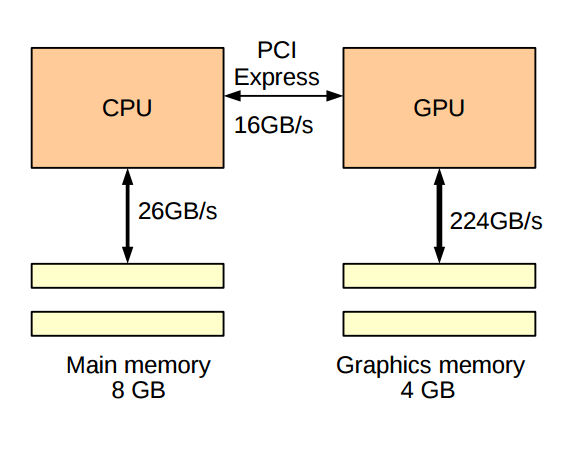
\includegraphics[width=.8\linewidth]{figures/memorygpu}
  \caption{GPU}
  \label{fig:sfig1}
\end{subfigure}%
\begin{subfigure}{.5\textwidth}
  \centering
  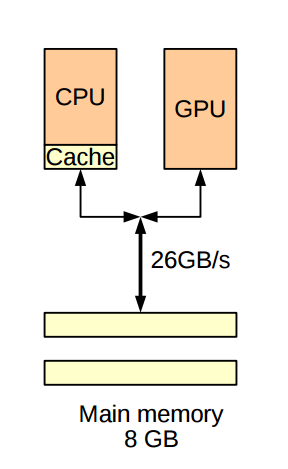
\includegraphics[width=.4\linewidth]{figures/memoryegpu}
  \caption{eGPU}
  \label{fig:sfig2}
\end{subfigure}
\caption{Memory organisation \cite{Collange2015}}
\label{fig:gpuegpu}
\end{figure}

Critical metrics of an eGPU for any application include functionality and its execution time. In the following thesis, a Stereo vision algorithm is chosen as a baseline, optimizations are done on the algorithm, and the metrics of an eGPU from ThinkSilicon called Nema are evaluated.\\

%%%%%%%%%%%%%%%%%%%%%%%%%%%%%%%%%%%%%
%%%%%%%%%%%%%%%%%%%%%%%%%%%%%%%%%%%%%
%%%%%%%%%%%%   SECTION   %%%%%%%%%%%%
%%%%%%%%%%%%%%%%%%%%%%%%%%%%%%%%%%%%%
%%%%%%%%%%%%%%%%%%%%%%%%%%%%%%%%%%%%%
\section{Problem Statement}
\label{sec:intro:probstatement}

Stereo vision is an active field with lot of ongoing research. There are many approaches for disparity map (DM) creation in a passive binocular Stereo vision system. The functional performance of an algorithm is highly dependent on the parameters chosen. Execution time of an algorithm is also a critical factor in a Stero vision application. A study of parameter variations and software optimizations on a Stereo vision algorithm are required for a better understanding of the algorithm. 

Think silicon Ltd. has developed a new version of eGPU called Nema. The GPU has to be tested out for a real world application. A suitable application for the eGPU could be a passive binocular Stereo vision system. An algorithm needs to be chosen for the Stereo vision application. The parameters of the algorithm need to be finalised. Possible software optimizations need to be done to improve the execution time of the algorithm. Further acceleration of the algorithm facilitated by the GPU needs to be measured. Any bottleneck causing reduction in the acceleration of the system needs to be identified and reasoned out.


%%%%%%%%%%%%%%%%%%%%%%%%%%%%%%%%%%%%%
%%%%%%%%%%%%%%%%%%%%%%%%%%%%%%%%%%%%%
%%%%%%%%%%%%   SECTION   %%%%%%%%%%%%
%%%%%%%%%%%%%%%%%%%%%%%%%%%%%%%%%%%%%
%%%%%%%%%%%%%%%%%%%%%%%%%%%%%%%%%%%%%
\section{Contributions}
\label{sec:intro:contrib}

Stereo vision is an active and one of the most heavily investigated areas of computer vision. One of the major applications of Stereo vision system is in autonomous robotics \cite{pinhas_ben-tzvi_embedded_2010}. In many applications under autonomous robotics, like drones, the size and the power consumption of the system plays an important role. eGPU based hardware provide a very good trade-off between the size, power and performance for embedded applications. Hence, investigation of a performance of eGPU running a Stereo vision algorithm serves as an important research topic.
%

In summary, the main contributions of this thesis are:

\begin{itemize}
\item{Algorithm choice and Optimizations}
  \begin{itemize}
    \item Choice of a Stereo vision algorithm and its parameters for the eGPU evaluation.
    \item Software optimizations of the algorithm for faster execution time.
    \item Measurement of functional and run-time performance of various versions of the algorithm in different hardware.
  \end{itemize}
\item {eGPU evaluation}
     \begin{itemize}
    \item Implementation of the algorithm in Nema eGPU.
    \item Report of functional verification and acceleration provided by eGPU
    \item Detecting and reasoning out of bottlenecks.
    \end{itemize}
\end{itemize}
%%%%%%%%%%%%%%%%%%%%%%%%%%%%%%%%%%%%%
%%%%%%%%%%%%%%%%%%%%%%%%%%%%%%%%%%%%%
%%%%%%%%%%%%   SECTION   %%%%%%%%%%%%
%%%%%%%%%%%%%%%%%%%%%%%%%%%%%%%%%%%%%
%%%%%%%%%%%%%%%%%%%%%%%%%%%%%%%%%%%%%
\section{Thesis outline}
\label{sec:intro:outline}

The rest of this thesis is organized as follows:

\begin{compactitem}
  \item Chapter 2 focuses on the background of Stereo vision. The hardware and software components of GPUs in general and Nema in particular are discussed. Kernel and mapping information of the eGPU is provided. Related work in the field are discussed.
  \item Chapter 3 discusses on the Stereo vision algorithm. It also provides information on various optimizations done on the algorithm.
  \item Chapter 4 discusses on the software implementation of the algorithm. Results of parameteric variations and execution time of various optimized versions of the algorithm in different hardware are presented. 
  \item Chapter 5 discusses on the eGPU implementation of the algorithm. The functionality and the execution time of the algorithm on the GPU is discussed. Comments on the eGPU based on the observations are presented.
  \item Chapter 6 provides the conclusion, suggestions for imrprovement. Future work in the lines are discussed.
\end{compactitem}

%%%%%%%%%%%%%%%%%%%%%%%%%%%%%%%%%%%%%%%%%%%%%%%%%%%%%%%%%%%%%%%%%%%%%%%%%%
%%%%%%%%%%%%   CHAPTER 2   %%%%%%%%%%%%%%%%%%%%%%%%%%%%%%%%%%%%%%%%%%%%%%%%
%%%%%%%%%%%%%%%%%%%%%%%%%%%%%%%%%%%%%%%%%%%%%%%%%%%%%%%%%%%%%%%%%%%%%%%%%%
\chapter{Background and Related work}
\label{chap:backgroundandrelatedwork}

%intro
%
This chapter initially discusses the background of Stereo vision, implementation platforms, Nema eGPU architecture, and kernel \& mapping information of the eGPU. Towards the end, current research done on the Stereo vision and GPU fields are discussed along with implication of their importance.


%%%%%%%%%%%%%%%%%%%%%%%%%%%%%%%%%%%%%
%%%%%%%%%%%%%%%%%%%%%%%%%%%%%%%%%%%%%
%%%%%%%%%%%%   SECTION   %%%%%%%%%%%%
%%%%%%%%%%%%%%%%%%%%%%%%%%%%%%%%%%%%%
%%%%%%%%%%%%%%%%%%%%%%%%%%%%%%%%%%%%%
\section{Stereo vision}
\label{s:stereovision}

Stereo vision involves extraction of depth information from multiple camera images of the same scene. The basic form of Stereo vision is binocular Stereo vision involving two cameras as shown in the Figure \ref{fig:bsv}. In the figure, it can be noticed that both the Left and the Right camera, take the image of a point P. These two cameras are separated by a distance b, called the baseline. The image planes of both the cameras are also shown in the figure. These image planes contain the pixel projections of the points in the scene for each of the cameras respectively. For example, the right camera sees the point P on the pixel U\textsubscript{R}, while the left camera sees the point P in the pixel U\textsubscript{L}. It can be seen that there is a shift along the X-axis while comparing the projections of the point in the two image planes. That is, in the above figure pixel U\textsubscript{R} is closer to the left end of the image plane while the pixel U\textsubscript{L} is closer to the right end.  This shift increases as the point P gets closer to the camera. Thus, if one can measure the shift in the position of the pixel for any point in the scene between the two image planes, the relative depth (disparity) of that point in the scene can be found out. An image giving disparity of all the points in the image plane is called disparity map (DM). The absolute depth can also be calculated if the focal lengths of the cameras are known.\\


\begin{figure}[!htbp]
    \center
    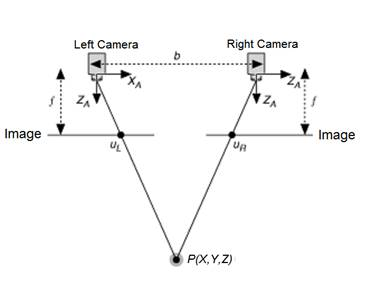
\includegraphics{figures/StereoVision}
    \caption{Illustration of binocular stereovision \cite{_3d_2013}.}
    \label{fig:bsv}
\end{figure}

This thesis deals with binocular Stereo vision (Stereo vision involving two cameras). In binocular Stereo vision, image from one of the cameras is taken. Then for each pixel in that image, the pixel corresponding to the same point in the scene is found in the image from the other camera. Then the positions of the two pixels in their respective image planes are compared in order to arrive at the depth of the point in the scene. In order to arrive at the depth, the cameras' geometry and properties need to be taken into account\\

\begin{figure}[!htbp]
    \center
    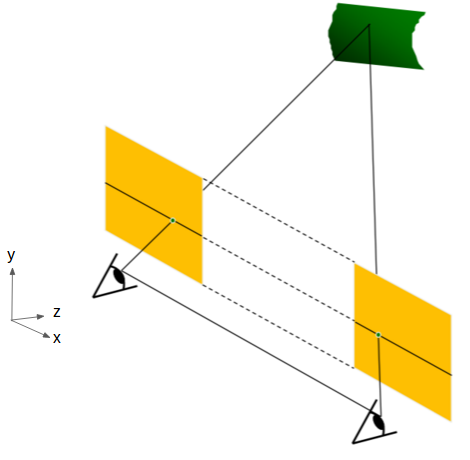
\includegraphics[width=75mm]{figures/Assumptions}
    \caption{Assumptions on stereovision set up \cite{derek_hoiem_epipolar_2011}.}
    \label{fig:assumptionssv}
\end{figure}

There are some assumptions made regarding the stereo images used in this thesis:
\begin{enumerate}
    \item The left and the right cameras used to take the images are synchronous i.e. the images from the left and the right cameras are taken at the same instant. This is in contrast with another method where a single camera takes image of a scene from multiple points at different instances of time.
    \item The image planes of the cameras used in taking images are coplanar.
    \item The reference axes of the image planes coincide.
    \item The centers of the cameras used to take the images are  in same height. The points 2,3 and 4 together imply that the image planes of the right and left cameras have the same reference axes x,y, and z and they are only shifted laterally along the x-axis (they are not rotated).
    \item The physical properties of the cameras, for example focal length and the resolution are the same.
\end{enumerate}

Samples of images used in this thesis complying with the given conditions are shown in the Figure \ref{fig:samplessv}.

\begin{figure}[!htbp]
\begin{subfigure}{.5\textwidth}
  \centering
  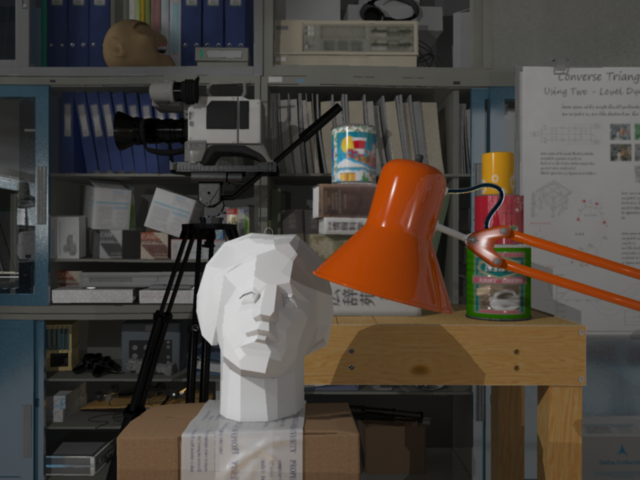
\includegraphics[width=.8\linewidth]{figures/frame_1_left}
  \caption{Tsukuba left}
  \label{fig:sfig1}
\end{subfigure}%
\begin{subfigure}{.5\textwidth}
  \centering
  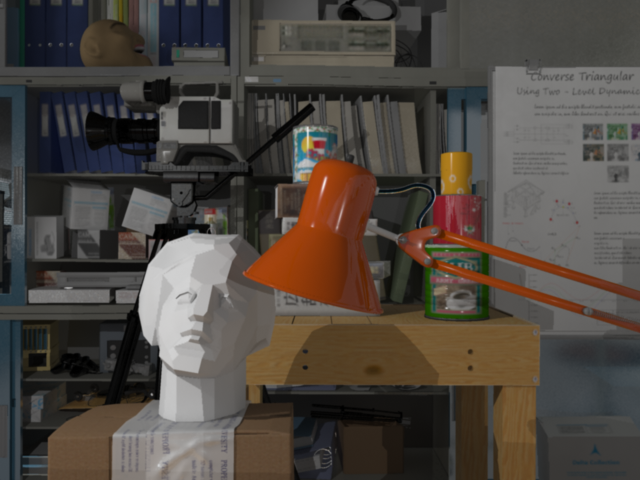
\includegraphics[width=.8\linewidth]{figures/frame_1_right}
  \caption{Tsukuba right}
  \label{fig:sfig2}
\end{subfigure}
\begin{subfigure}{.5\textwidth}
  \centering
  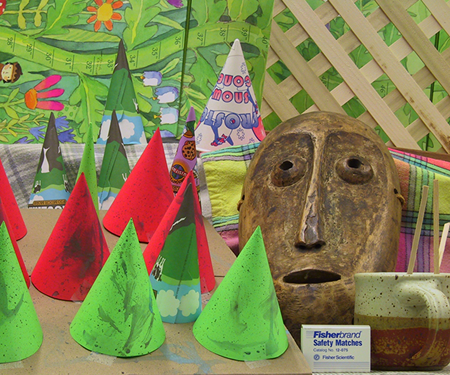
\includegraphics[width=.8\linewidth]{figures/ConeL}
  \caption{Middlebury left}
  \label{fig:sfig3}
\end{subfigure}%
\begin{subfigure}{.5\textwidth}
  \centering
  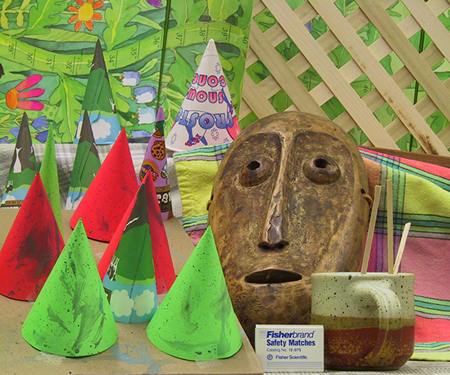
\includegraphics[width=.8\linewidth]{figures/ConeR}
  \caption{Middlebury right}
  \label{fig:sfig4}
\end{subfigure}
\begin{subfigure}{.5\textwidth}
  \centering
  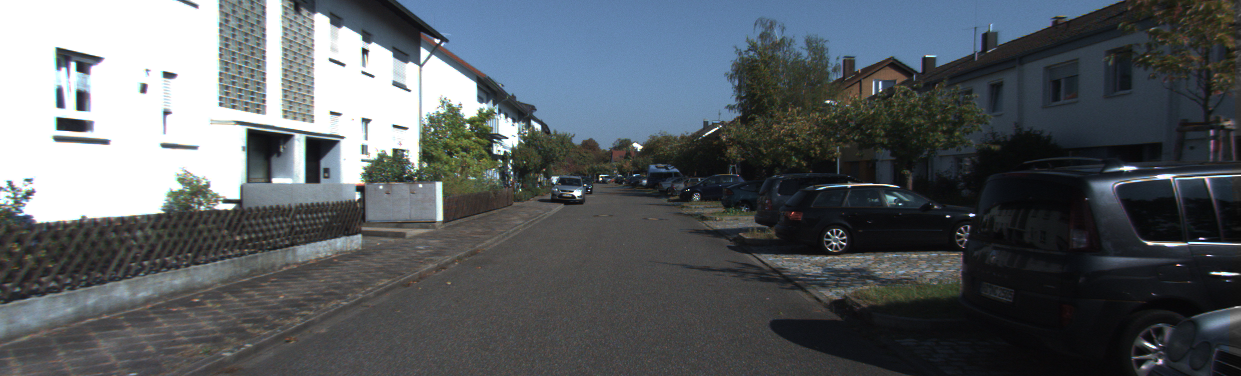
\includegraphics[width=.8\linewidth]{figures/RoadL}
  \caption{KIT left}
  \label{fig:sfig5}
\end{subfigure}%
\begin{subfigure}{.5\textwidth}
  \centering
  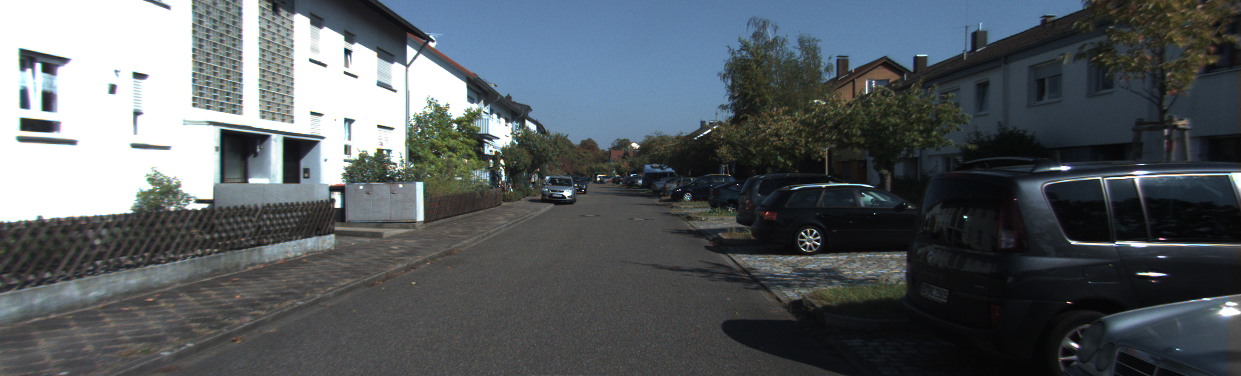
\includegraphics[width=.8\linewidth]{figures/RoadR}
  \caption{KIT right}
  \label{fig:sfig6}
\end{subfigure}
\caption{Sample Stereo vision images}
\label{fig:samplessv}
\end{figure}

%%%%%%%%%%%%%%%%%%%%%%%%%
%%%%%   SUB-SECTION   %%%
%%%%%%%%%%%%%%%%%%%%%%%%%
%%%%%%%%%%%%%%%%%%%%%%%%%
\subsection{Disparity Map evaluation}
\label{s:stereovision:bmpre}

The quality of the DM obtained by an algorithm is decided by its comparison with the ground truth. There are many methods of error estimation of a DM with respect to ground truth. In this thesis, Bad Matched Pixels Relative Error (BMPRE) method proposed by Cabezas et al. \cite{Cabezas2012} is used for the error estimation and hence the functional verification of the algorithm across parameters. With the ground truth available, the relative error of each pixel with respect to the true disparity value sheds light on how good the algorithm's performance is in estimating the depth values. The BMPRE method considers these aspects during the error evaluation and is hence chosen.

The BMPRE measure is formulated as:

\begin{equation}
 BMPRE =\sum\nolimits_{(x,y)}^{N}
   \begin{cases}
    \tau(x,y)       & \quad \text{if } \Delta({\rm x}, {\rm y}) > \delta\\
    0  & \quad \text{if } \Delta({\rm x}, {\rm y})\leq \delta\\
  \end{cases}
  \label{eqn:bmpre}
\end{equation}

where $\Delta(x,y)$ is the absolute difference between the obtained disparity and the ground truth at coordinates (x,y) $\delta$ is the threshold for error and $\tau(x,y)$ is given by:
\[
  \tau({\rm x}, {\rm y})=
  \begin{cases}
    \Delta(x,y)\over {D}_{true}(x,y)       & \quad \text{if } {D}_{true}(x,y) > 0\\
    0  & \quad \text{if } \text{otherwise}\\
  \end{cases}
\]

Here ${D}_{true}(x,y)$ indicates the disparity value of the ground truth at position (x,y). In the current thesis $\delta$ value of 2 is chosen for the calculation. The choice of $\delta$ is arbitrary as the performace of same algorithm across parameters is compared.

%%%%%%%%%%%%%%%%%%%%%%%%%%%%%%%%%%%%%
%%%%%%%%%%%%%%%%%%%%%%%%%%%%%%%%%%%%%
%%%%%%%%%%%%   SECTION   %%%%%%%%%%%%
%%%%%%%%%%%%%%%%%%%%%%%%%%%%%%%%%%%%%
%%%%%%%%%%%%%%%%%%%%%%%%%%%%%%%%%%%%%
\section{GPU hardware}
\label{s:gpuhw}

%
The ALUs in GPU are simpler in nature compared to those in CPUs. A particular ALU in a GPU takes more time for execution of a single instruction compared to an ALU in a CPU. Thus, CPU is said to be latency optimised compared to GPU. However, GPUs have a huge number of ALUs for each core (or multiprocessor) compared to CPUs. This means that all the ALUs can work at the same time thus increasing the throughput. Overall, this makes the GPU much faster for parallelizable problems. CPUs are low latency low throughput devices while GPUs are high latency high throughput devices. The architecture of GPU in comparison with CPU is as shown in the Figure \ref{fig:cpugpu}.

\begin{figure}
    \center
    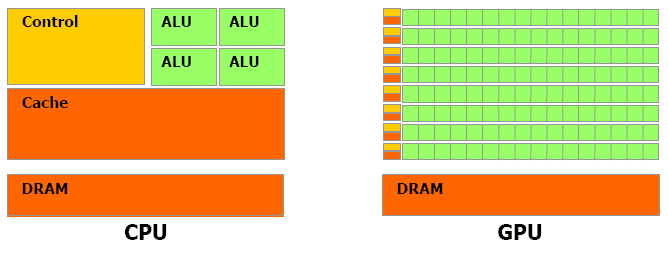
\includegraphics[width=.8\linewidth]{figures/cpugpu}
    \caption{Architecture comparison between CPU and GPU \cite{gpu2008}.}
    \label{fig:cpugpu}
\end{figure}


%%%%%%%%%%%%%%%%%%%%%%%%%
%%%%%   SUB-SECTION   %%%
%%%%%%%%%%%%%%%%%%%%%%%%%
%%%%%%%%%%%%%%%%%%%%%%%%%
\subsection{Nema hardware}
\label{s:gpuhw:nema}

Nema is an embedded GPU platform designed by ThinkSilicon taking low energy consumption and silicon footprint into consideration \cite{_nema|s}. It is scalable many-core, multi-threaded design with both graphics rendering and general computing capabilities. It is deployed in a reusable soft IP core suitable for ASIC or FPGA implementation. Nema GPU employs multiple processing cores in clusters, and multiple clusters can be connected via a proprietary network-on-chip (NoC). This along with a memory subsystem design allows Nema to be scaled to a multi-core GPU of a size required by the problem in hand. Software development for Nema can be done through industry-standard APIs supported by a dedicated LLVM/Clang compiler toolchain which adapts to the changing architecture. Nema currently supports C/C++ programming. The Figure \ref{fig:nemaarch} shows the generic architecture of Nema GPU.

\begin{figure}
    \center
    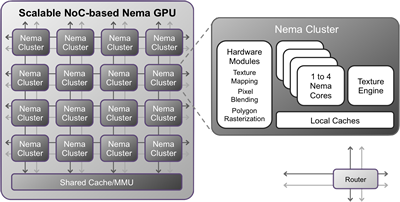
\includegraphics[width=75mm]{figures/nema_diagram}
    \caption{Nema GPU architecture \cite{_nema|s}.}
    \label{fig:nemaarch}
\end{figure}

The implementation of the system is done in zc706 evaluation board from Xilinx. The eGPU is deployed in the FPGA of the Zync7000 processor. The implementation of Nema in this thesis involves 4 cores with 16 threads each. The cores together have a common data cache of 1 MB. The threads are 32 bit. Nema implemented on Zynq 7000 runs with a frequency of 83 MHz.

%


%%%%%%%%%%%%%%%%%%%%%%%%%%%%%%%%%%%%%
%%%%%%%%%%%%%%%%%%%%%%%%%%%%%%%%%%%%%
%%%%%%%%%%%%   SECTION   %%%%%%%%%%%%
%%%%%%%%%%%%%%%%%%%%%%%%%%%%%%%%%%%%%
%%%%%%%%%%%%%%%%%%%%%%%%%%%%%%%%%%%%%
\section{GPU software}
\label{s:gpusw}

GPUs use SIMD (single instruction multiple data) model of programming. They execute the same instructions on different data. The large data set on which the GPU operates is called the stream \cite{Rege}. The set of instructions which operate on each datum is called kernel or shader \cite{Rege}. Each instance of the kernel on a particular ALU is called the thread.

The term shader is used to refer to a kernel as traditionally GPUs were employed for graphic applications. A common application is to render a complete object taking a set of its vertices as inputs. The components of GPU programming are named after the components in graphic rendering. The main parts of GPU programming include blender, rasterizer and interpolators. The blender takes care of the shading environment, like the physical address of the frame buffer (monitor), the colour mode of the shading and the viewport of the image. Rasterizer is responsible for discretising the portions of the object for rendering. For example the object can be a sphere, which is a continuous set of points. However the display environment consists of pixels, a discrete set of points. Rasterizer takes care of the discretization of the sphere so that it can be displayed as an image. A general case is that each thread in a GPU is responsible for each pixel in an image. Hence rasterizer's function can be considered as the deployment of threads in the GPU. Interpolator traditionally is responsible for calculating the colour at a coordinate discretized by rasterizer based on colour at known vertices. In this thesis interpolators are used to calculate the memory locations of the input pixels. The general function of rasterizer and interpolator is as illustrated in the Figure \ref{fig:rastint}.

\begin{figure}
    \center
    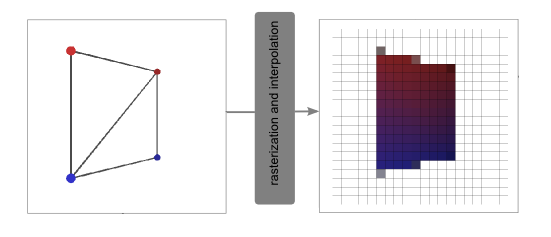
\includegraphics[width=.8\linewidth]{figures/rastint}
    \caption{Function of Rasterizer and Interpolator \cite{Colubri}.}
    \label{fig:rastint}
\end{figure}

%%%%%%%%%%%%%%%%%%%%%%%%%
%%%%%   SUB-SECTION   %%%
%%%%%%%%%%%%%%%%%%%%%%%%%
%%%%%%%%%%%%%%%%%%%%%%%%%
\subsection{Programming Nema}
\label{s:gpusw:nema}

The programming of Nema GPU is done by writing to hardware registers \cite{Apostolou2015}. The values in these register control the workflow of Nema. In C\textbackslash C++Access to these registers is provided by libNemaUtils.so library. The library includes functions to read\textbackslash write to registers and synchronization functions. Like every other C++ library, the libNemaUtils.so needs to be linked with the corresponding header files included for proper function of the host code. The method used for programming Nema is command list method. Commands list consists of a batch of register writes which correspondingly programs the GPU components like blender and rasterizer. Once the command list is ready, it is flushed to the GPU. While the GPU performs the tasks defined by the command list the CPU can continue preparing new command list.

Nema operates on contiguous memory locations. The blender and rasterizer of Nema usually are programmed once for an application. The programming parameters of the blender include starting address, frame buffer stride, frame buffer resolution, viewport and blending mode. The rasterizer is responsible for generating the threads in the GPU. The parameters of Rasterizer include the coordinates of the starting and the ending thread.

Nema includes interpolators that can be programmed to generate values according to the thread coordinates. There are four interpolators available in Nema. Each can be programmed with a starting value step and stride. The values then generated in each GPU thread can be used by the thread for coordinate specific operations. For example, the memory locations of the pixel in the images can be generated by interpolators. Nema also includes constant registers to store the values which remain constant across all GPU threads.The memory space of Nema is managed by nema\_malloc() function. This uses Nema's custom memory manager to ensure that contiguous memory locations are allocated for proper functionality of Nema. The functionality of nema\_malloc() is very similar to that of standard malloc() function. This operates on virtual memory addresses. While transferring the memory location to Nema it needs to be converted to physical address.

nema\_wait\_for\_status() and nema\_wait\_for\_interrupt() are used for synchronization between the host cpu and the gpu. The first functions performs a busy wait polling on the gpu's status register checking if the GPU has completed operation. The second function puts the calling process into a sleep state until the gpu
 raises an interrupt.

%%%%%%%%%%%%%%%%%%%%%%%%%
%%%%%   SUB-SECTION   %%%
%%%%%%%%%%%%%%%%%%%%%%%%%
%%%%%%%%%%%%%%%%%%%%%%%%%
\subsection{Nema kernels}
\label{s:gpusw:nkernels}

 Parallelisable part of the code are written as C kernels in Nema. Each kernel in Nema has access to the interpolater values to perform the particular thread dependent operations. The thread also has access to it's coordinates. Nema also has 16 constant vector registers, meaning 16 registers with 4 32bit element each. An example of kernel is shown in the Appendix \ref{s:kerero}. The read\_reg() function is used to read the constant and interpolator values by each instance of the kernel. The read\_coords() function provides the coordinates of the particular instance of the kernel. These values serve as inputs and outputs for the kernel instance. The kernels are compiled by custom script from ThinkSilicon to generate a .bin file. This .bin file is then loaded into the Nema by the host program during run-time. An example of the host program is provided in the Appendix \ref{s:hostero}. Nema kernels do not have synchronization facilities between the cores. This implies that the threads run independent of each other. Simplified programming structure of Nema eGPU is shown in the Figure \ref{fig:kernelstruct}. The figure indicates the program and data flow between the host and the device (eGPU).

 \begin{figure}
    \center
    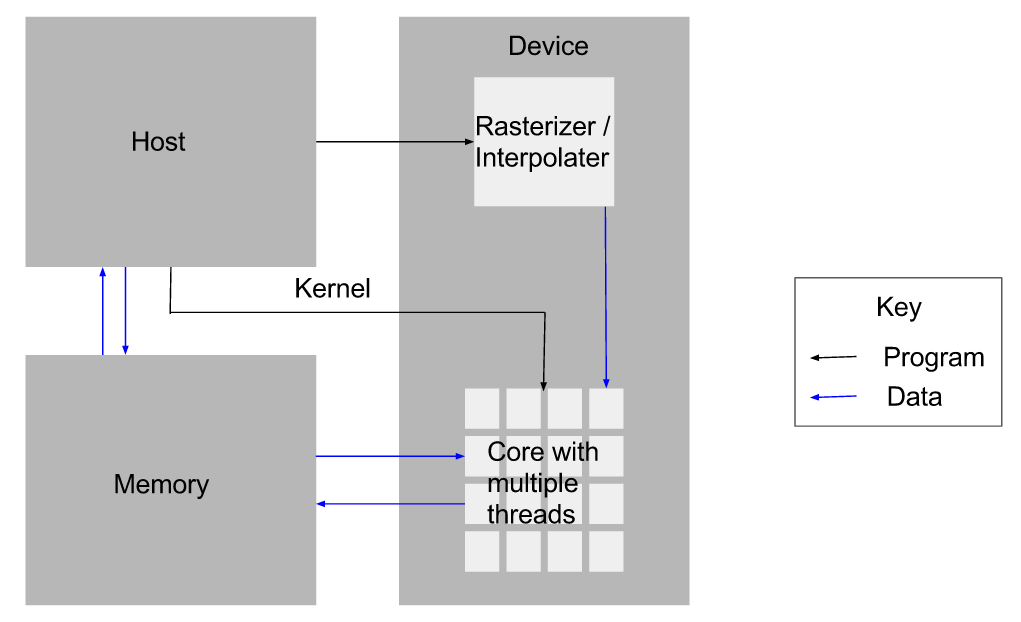
\includegraphics[width=.8\linewidth]{figures/kernelstruct}
    \caption{Simplified program structure in Nema eGPU.}
    \label{fig:kernelstruct}
\end{figure}

%%%%%%%%%%%%%%%%%%%%%%%%%%%%%%%%%%%%%
%%%%%%%%%%%%%%%%%%%%%%%%%%%%%%%%%%%%%
%%%%%%%%%%%%   SECTION   %%%%%%%%%%%%
%%%%%%%%%%%%%%%%%%%%%%%%%%%%%%%%%%%%%
%%%%%%%%%%%%%%%%%%%%%%%%%%%%%%%%%%%%%
\section{Related work}
\label{s:rwork}
A lot of research is done in Stereo vision involving GPUs. GPUs serve as a reliable parallel platform for algorithms such as Stereo vision. They have a fixed architecture and are not limited by space constraints in contrast to FPGAs \cite{Kalarot2010}. In this section some of research done regarding Stereo vision implementation in GPUs are discussed.\\

In \cite{Xu2014}, T. Xu et al. present accelerated version of a Stereo vision algorithm for multi-core CPU and GPU. The evaluated algorithm, the Parallel Pyramid Matcher algorithm, finds application in clothes folding robot. The algorithm is broken down into several subatomic algorithm to understand the performance acceleration. The single core Java implementation (Single Instruction Single Data (SISD)) is compared against Vector Pascal (multi-core) and C\textbackslash C++ \& CUDA implementation (GPU). The experiments were conducted in three different multi-core architectures; AMD Opteron 6366HE, Intel Xeon E5-2440, and Intel Xeon E5-2620; and Nvidia GeForce GTX 770 GPU. One of the interesting findings in the experiment shows a slight increase in execution time of the algorithm in 64 core AMD architecture when the number of threads go beyond 30. This is in contrast with Amdahl's law which expects the execution time to keep decreasing with increase in number of threads provided there is hardware support. The observation is explained by increase in allocation time for threads as the number of used cores increases. Experiments further revealed a 12x speed up in multi-core architecture and 176x speed up with GPU compared to the SISD implementation. The sub-algorithm providing the maximum speed-up was also identified.

Y. Choi et al. propose Graph Cut (GC) based on GPUs for Stereo matching \cite{Choi2013}. The problem of DM creation was approched as a directed graph problem. The method used by Kolmogorov \cite{Kolmogorov2004} is used to construct graphs. Stereo matching is modelled as a multi-label graph problem and is broken down into a series of bi-label problems. Then each bi-label problem is solved using GC. The algorithm is modified to minimized the kernel loading overhead, and to increase the number of computations for global to shared memory transfer in the GPU. Experiments show that 5.2X speedup is obtained in execution time with 0.12\% degradation in accuracy compared to conventional GPU implementation.

Acceleration of SymStereo algorithm using GPU was experimented in \cite{Mota2014}. Unlike conventional Stereo matching algorithms, SymStereo algorithm uses symmetry to evaluate the likelihood of two pixels matching. Generally, Stereo matching can be divided into two parts: creating a disparity space image (DSI) using matching cost functions, and evaluation of DSI to create depth maps. In this paper V. Mota et al. work on accelerating the creation of DSI. Experiments were done on Nvidia Geforce GTX 680 GPU using CUDA 5.0. Across parameters of the algorithm, it was found that they were able to process low-resolution images 53 fps and high-resolution images in 3 fps.

A comparison of FPGA and GPU implementation of real-time Stereo vision was done in \cite{Kalarot2010}. Symmetric Dynamic Programming Stereo (SDPS) is used for the comparison in this paper. Unlike conventional Stereo matching algorithms which create DMs for the right or the left image, SDPS creates a DM for a virtual camera midway between the two cameras. The algorithm is modified to fit the architecture of Altera Stratix III FPGA and Nvidia GTX 280 GPU. It was found that despite a lower clocking rate of the FPGA, it was superior in performance compared to the GPU. The speed-up of FPGA is accounted to the deep extensive pipeline which enables transfer of results from the intermediate stages immediately. The slowdown of GPU was accounted to its internal overheads. It was found however that the bus input\textbackslash output time in the GPU was not a significant contributor to the execution time. It was also found that the FPGA has space limitations with increasing disparity ranges for SDPS algorithm.

\subsection{Summary}
\label{s:rwork:summary}
Intensive research is being done on Stereo vision systems. The focus of the research lies in increasing the accuracy of the system while minimising the execution time. GPUs are evolving as popular implementation platforms for Stereo vision systems. The simpler programming model of GPUs favours them over FPGAs. Algorithms are continually being modified to fit the GPU architecture without sacrificing much of the accuracy of the system. Current research work mostly involves conventional GPUs with a large number of cores. It would be insightful to implement and evaluate a Stereo vision system on an embedded GPU.
%%%%%%%%%%%%%%%%%%%%%%%%%%%%%%%%%%%%%%%%%%%%%%%%%%%%%%%%%%%%%%%%%%%%%%%%%%
%%%%%%%%%%%%   CHAPTER 3   %%%%%%%%%%%%%%%%%%%%%%%%%%%%%%%%%%%%%%%%%%%%%%%%
%%%%%%%%%%%%%%%%%%%%%%%%%%%%%%%%%%%%%%%%%%%%%%%%%%%%%%%%%%%%%%%%%%%%%%%%%%
\chapter{The Proposed Algorithm}
\label{chap:algorithm}

This chapter deals with the choice of the algorithm and the software optimizations done to it. The requirements of the algorithm are listed. Various components of the algorithm are explained. Software optimizations done to the algorithm to improve the execution time are explained. The final optimized version of the algorithm is presented and elaborated.


%%%%%%%%%%%%%%%%%%%%%%%%%%%%%%%%%%%%%
%%%%%%%%%%%%%%%%%%%%%%%%%%%%%%%%%%%%%
%%%%%%%%%%%%   SECTION   %%%%%%%%%%%%
%%%%%%%%%%%%%%%%%%%%%%%%%%%%%%%%%%%%%
%%%%%%%%%%%%%%%%%%%%%%%%%%%%%%%%%%%%%
\section{Algorithm requirements}
\label{s:requirements}

A binocular stereovision, as discussed in the Chapter \ref{chap:backgroundandrelatedwork}, involves taking each pixel in an image (for example left image), finding the corresponding pixel in the other image (right image), and finding the shift of the pixel between images. Considering the assumptions made in the Section \ref{s:stereovision} and the architecture of Nema GPU, the algorithm has a set of requirements to produce a reliable DM:
\begin{enumerate}
    \item The variations in the image due to reflections need to be reduced. Light from distant light sources reflects off different points in the scene before reaching the left and the right cameras. This will result in variations in the images as illustrated in the Figure \ref{fig:reflection}. These variations need to be reduced.
    \item The noise and gain of each camera need to be accounted for and normalised. Though the physical properties of the camera like focal length and resolution are assumed to be same, the image sensor of each camera might vary in performance. This might result in a certain point in the scene seeming brighter, for example, in one of the cameras compared to another. Such differences in the left and right images need to be reduced.
    \item In order to ease the GPU implementation, the algorithm is preferred to operate on integer variables. Nema GPU has the data size of 32 bits and the normal GPU functionality produces results to be written to the frame buffer of the display (32-bit pixels). Hence, it is desirable that the algorithm also produces results in integer format.
    \item The algorithm must be easily translatable for GPU implementation. It should be compatible with the kernel structure discussed in the Chapter \ref{chap:backgroundandrelatedwork}.
    \item The algorithm needs to be optimised as much as possible for run-time prior to GPU implementation. In order to narrow down any reduction in performance due to GPU bottleneck, this is desirable.
\end{enumerate}

\begin{figure}
\begin{subfigure}{.5\textwidth}
  \centering
  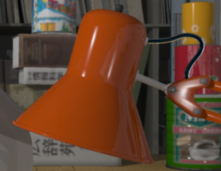
\includegraphics[width=.6\linewidth]{figures/reflectionleft}
  \caption{Left camera image}
  \label{fig:sfrl}
\end{subfigure}%
\begin{subfigure}{.5\textwidth}
  \centering
  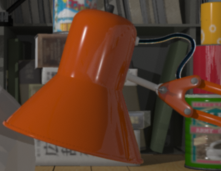
\includegraphics[width=.6\linewidth]{figures/reflectionright}
  \caption{Right camera image}
  \label{fig:sfrr}
\end{subfigure}
\caption{Reflection of light from distant light source}
\label{fig:reflection}
\end{figure}



%%%%%%%%%%%%%%%%%%%%%%%%%%%%%%%%%%%%%
%%%%%%%%%%%%%%%%%%%%%%%%%%%%%%%%%%%%%
%%%%%%%%%%%%   SECTION   %%%%%%%%%%%%
%%%%%%%%%%%%%%%%%%%%%%%%%%%%%%%%%%%%%
%%%%%%%%%%%%%%%%%%%%%%%%%%%%%%%%%%%%%
\section{Algorithm}
\label{s:algorithm}

The algorithm chosen for the evaluation addresses the stated requirements. The noise and gain of the camera are normalised by taking the census transform of both images. In order to reduce the variations in the image, the morphological transformation is applied. The chosen algorithm operates on integer variables. The compliance of the next two requirements will be evident as this chapter progresses. The algorithm chosen operates on monochrome versions of the images. The algorithm is split into two parts: Preprocessing and DM calculation as shown in the Figure \ref{fig:algorithmstructure}.

\begin{figure}
    \center
    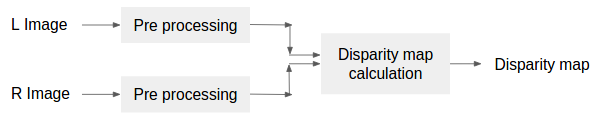
\includegraphics[width=.8\linewidth]{figures/algorithm_structure}
    \caption{Algorithm structure.}
    \label{fig:algorithmstructure}
\end{figure}
%

%%%%%%%%%%%%%%%%%%%%%%%%%
%%%%%   SUB-SECTION   %%%
%%%%%%%%%%%%%%%%%%%%%%%%%
%%%%%%%%%%%%%%%%%%%%%%%%%
\subsection{Preprocessing}
\label{s:algorithm:preprocessing}

The preprocessing stage involves reducing noise and variations between the two cameras. Variations in the images due to reflections is tackled by the morphological opening of each of the images \cite{Rosli2014}. The morphological opening consists of two parts: Morphological erosion, and Morphological dilation. Morphological erosion by any structure assigns the lowest value in the structure to the centre pixel. For a 3x3 square structure, morphological erosion at a pixel involves assigning the lowest value among the neighbouring pixels to that pixel as shown in the Figure \ref{fig:morphologicalerosion}.

 \begin{figure}
    \center
    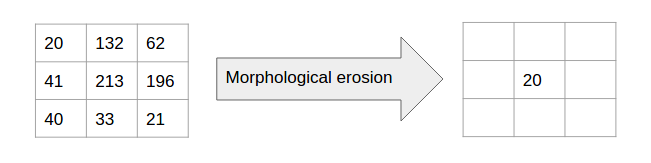
\includegraphics[width=120mm]{figures/Morphological_erosion}
    \caption{Morphologial erosion.}
    \label{fig:morphologicalerosion}
\end{figure}


Similarly, morphological dilation by any structure assigns the highest value in the structure to the centre pixel. For a 3x3 square structure, morphological dilation at a pixel involves assigning the highest value among the neighbouring pixels to that pixel as shown in the Figure \ref{fig:morphologicaldilation}.

 \begin{figure}
    \center
    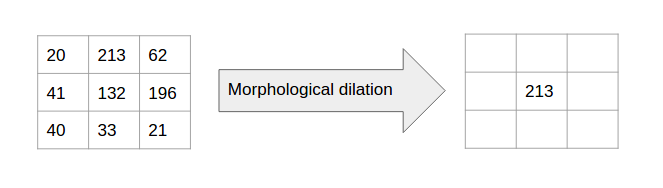
\includegraphics[width=120mm]{figures/Morphological_dilation}
    \caption{Morphologial dilation.}
    \label{fig:morphologicaldilation}
\end{figure}

Morphological erosion followed by dilation is called morphological opening and it is known to reduce white blobs in the image \cite{Rosli2014}. Thus, effects due to reflection on each image are reduced consequently reducing the variations between them.

The normalisation of the gain and the noise of cameras is done by census transform \cite{Zabih1994}\cite{young_ki_baik_fast_2006}. Census transform of a pixel P(x,y) is given by the Equation \ref{eqn:censustransform}.

\begin{equation}
  C(P) = \underset{[i,j]\in W}{\otimes} {\xi (P(x,y),P(x+i,y+j))} 
  \label{eqn:censustransform}
\end{equation}

Here $\bigotimes$ denotes concatenation, W denotes window of operation around P and $\xi$ is given by 

\[ \xi (P(x,y),P(x+i,y+j)) =
  \begin{cases}
    1       & \quad \text{if } P(x,y)>P(x+i,y+j)\\
    0  & \quad \text{if } \text{otherwise}\\
  \end{cases}
\]

\begin{figure}[!htbp]
    \center
    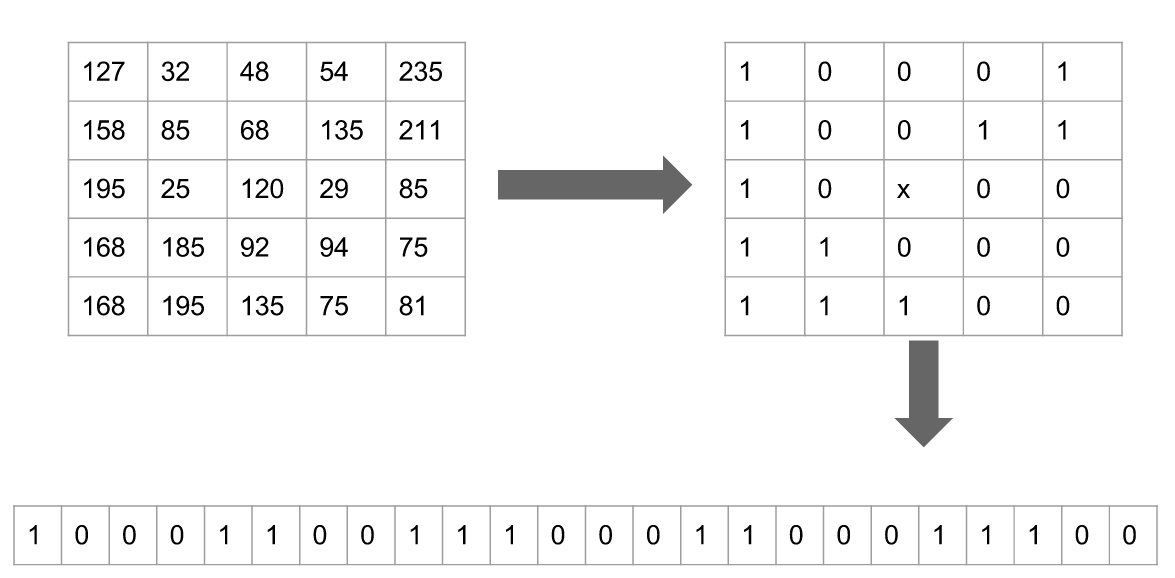
\includegraphics[width=.8\linewidth]{figures/Censustransform_example}
    \caption{Census transform example for 5x5 window.}
    \label{fig:censusexample}
\end{figure}

An example of a census transform for a 5x5 window around a pixel is as shown in the Figure \ref{fig:censusexample}. A census transformed image is invariant under changes in gain and bias \cite{young_ki_baik_fast_2006}. Hence, it can be used for normalisation of gains of both cameras.

%%%%%%%%%%%%%%%%%%%%%%%%%
%%%%%   SUB-SECTION   %%%
%%%%%%%%%%%%%%%%%%%%%%%%%
%%%%%%%%%%%%%%%%%%%%%%%%%
\subsection{Disparity Map calculation}
\label{s:algorithm:dmcalculation}

For the purpose of DM calculation, Sum of Hamming Distances (SHD) algorithm is used. This algorithm is chosen as it has the best speed performance in parallel architecture like FPGA or GPU \cite{GyorgyTamasBiroKaroly-Agoston2015}. It is a window based comparison technique. Here a window of pixels around each pixel in one image (left) is compared for a match in the other image (right). Generally, window based comparison algorithm assume all pixels in the window have a similar disparity value \cite{Hamzah2015}. However, this is not true. Hence, there is a poor performance in the regions where there is a large change in disparity values within a window. SHD algorithm is known to be robust against this issue \cite{Hamzah2015}. SHD between two census transformed pixels is calculated by XORing each bit of all the pixels within a window of a particular size around the pixels, and summing the result up. Mathematically SHD at a pixel x,y can be expressed as shown in the Equation \ref{eqn:shd}.

\begin{equation}
  SHD(x,y,D) = \underset{[i,j]\in W}{\sum} {{\sum_{\substack{bits}}}XORbitwise\big(P(x+i,y+j),Q(x+i-D,y+j)\big)} 
  \label{eqn:shd}
\end{equation}

Here P is the reference image(left image), Q is the target image(right image), W denotes window of operation and D denotes the disparity level.\\
Disparity of a particular pixel
\begin{equation}
  DM(x,y) = \underset{D\in [a..b]}{argmin}{\big(SHD(x,y,D)\big)}
  \label{eqn:dm}
\end{equation}

where D is the range of disparity levels with a and b as minimum and maximum values respectively.

In the current thesis, 3x3 square structure is used for morphological opening, 11x11 window is used for census transform and 13x13 window is used for DM calculation. The disparity levels range from 0 to 100. The choice of these values is explained in Chapter 4.


%%%%%%%%%%%%%%%%%%%%%%%%%%%%%%%%%%%%%
%%%%%%%%%%%%%%%%%%%%%%%%%%%%%%%%%%%%%
%%%%%%%%%%%%   SECTION   %%%%%%%%%%%%
%%%%%%%%%%%%%%%%%%%%%%%%%%%%%%%%%%%%%
%%%%%%%%%%%%%%%%%%%%%%%%%%%%%%%%%%%%%
\section{Optimizations}
\label{sec:optimizations}

The algorithm is implemented in C\textbackslash C++ and run on various PCs. The first version of the algorithm is implemented in Matlab to ensure its functionality. Subsequent versions are implemented in C++. The png++ library is used for image input and output. Various optimizations done on the initial C++ version to improve the execution time are discussed in this section. The results of each optimization on different platforms is presented in the next chapter.

\subsection{Datastructure optimization}
\label{s:optimizations:dsoptimization}

\begin{figure}[!htbp]
    \center
    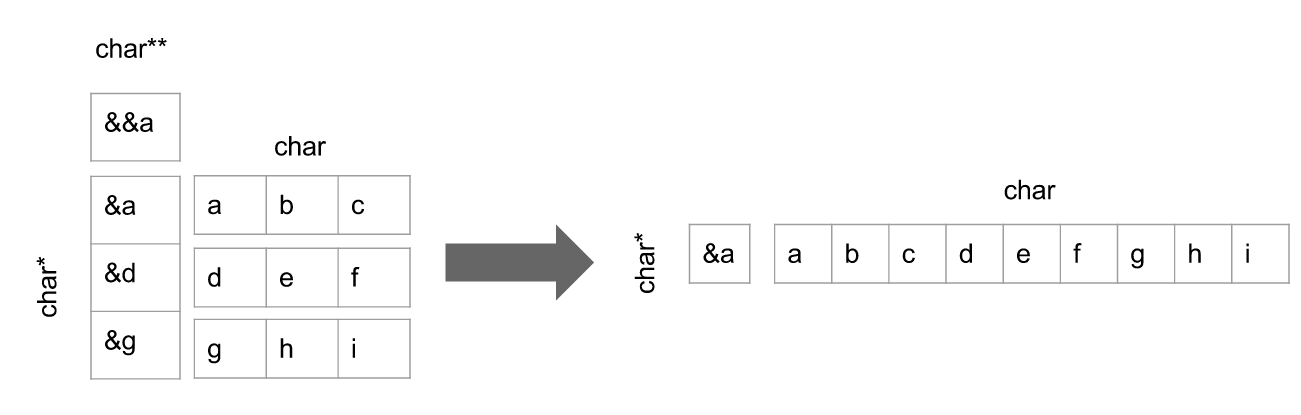
\includegraphics[width=.8\linewidth]{figures/dsoptimization}
    \caption{Datastructure optimization.}
    \label{fig:dsoptimization}
\end{figure}

The initial C++ version of the algorithm stores unprocessed images in 2D arrays. The elements of the array are referenced by a char** pointer. Manipulating and dereferencing a char** pointer gives a char* pointer or the row of an element in the array. The char* pointer, in turn, can be manipulated and dereferenced to reveal an element of the array. It is clear that in order to access a particular pixel of the image (element of the array) two levels of dereferencing needs to be done. This can be reduced to a single level dereferencing by replacing the 2D arrays by pseudo-2D arrays \cite{Souli2007}. Now the data structure of an unprocessed image is a 1D array. Now every pixel can be directly accessed from the memory using char* datatype. The same optimization is done for different versions of the image reducing the number of dereferences and hence improving the run-time performance. This optimization is illustrated in the Figure \ref{fig:dsoptimization} for a 3x3 array.

\subsection{Multithreading}
\label{s:optimizations:multithreading}

The DM calculation part of the algorithm chosen is parallelizable. This is because the calculation of DM at any pixel is independent of the DM calculation at another pixel. Many implementation platforms have a multi-core capability. This advantage provided by the platform can be utilised in order to speed up the algorithm \cite{threadcpp}. The images are split into four sections and the DM calculation at each part of the image is issued as a different thread. This allows parallel execution of the algorithm and leads to improvement in run-time performance.

\subsection{Invariant code motion}
\label{s:optimizations:invariantcodemotion}

\begin{figure}[!htbp]
    \center
    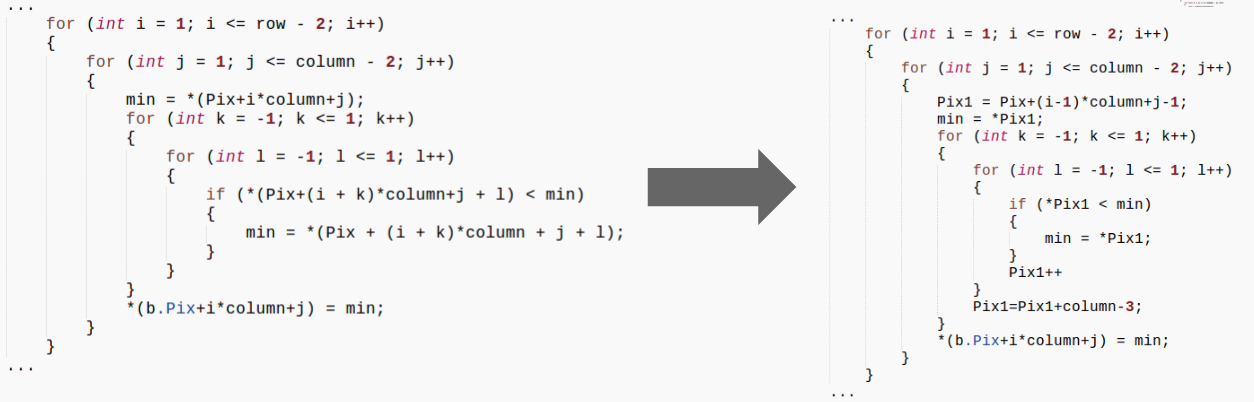
\includegraphics[width=\linewidth]{figures/icmoptimization}
    \caption{Invariant code motion optimization.}
    \label{fig:icmoptimization}
\end{figure}

DM calculation in the algorithm involves multiple loops with pointer manipulation and dereferencing inside the innermost loop. This involves calculation of address of a pixel every iteration involving multiple operations. Since most of the calculations happen between consecutive pixels, if the address of the current pixel is stored and incremented, it can be used to access the required pixel in the next iteration \cite{Aho2006}. One other way of seeing this is that iteration variables of the outer loop remain invariant in the innermost loop and hence the calculations involving can be moved outside the loop and stored. This optimization works well if the hardware has enough registers to store the newly created variables. In case, the hardware does not contain enough registers the variables might get spilled. The case of insufficient registers could also happen due to the execution of multiple threads of the same function, creating a need for more variables. Invariant code motion optimization is illustrated in the Figure \ref{fig:icmoptimization}. Here one can notice that by creating a variable Pix1 in loop 2, one can save a lot of calculations on Pix in loop 4. This is replaced by a simple increment on Pix1.

\subsection{SIMD}
\label{s:optimizations:simd}
Census transform with an 11x11 window for each pixel results in a 120-bit value. This is stored in two long integers(64 bit each). During the DM calculation, XOR operation is performed on these data between two images. One can notice that the same operation is performed on multiple variables(two long integers) for each pixel. This can be accelerated using the vectorization techniques offered by the processor \cite{Siewert2009}. The resulting implementation produces just one operation(128 bit XOR) for each pixel instead of two. Acceleration obtained by this SIMD(single instruction multiple data) operation is studied.

\subsection{Store and reuse of XOR values}
\label{s:optimizations:xoroptimization}

\begin{figure}[!htbp]
    \center
    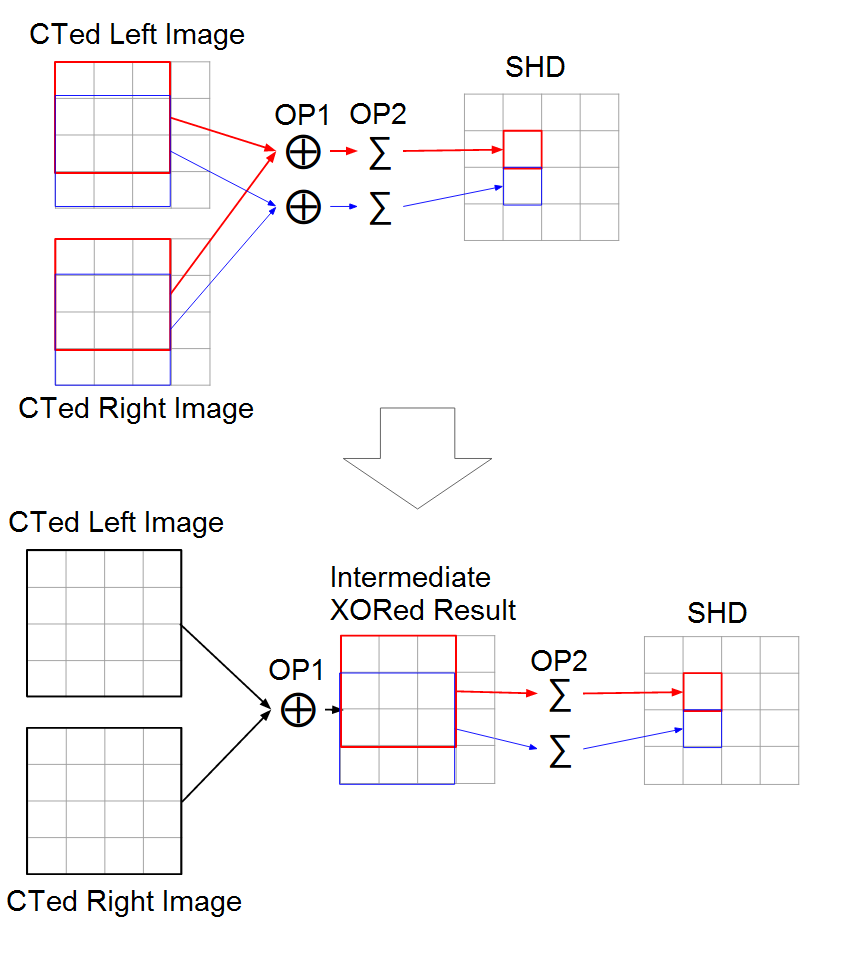
\includegraphics[width=.8\linewidth]{figures/xoroptimization}
    \caption{Storage and reuse of XOR values.}
    \label{fig:xoroptimization}
\end{figure}

The formula for SHD calculation is given in the Equation \ref{eqn:shd}. For an arbitrary position (x,y), the sum of bits in bitwise XOR is performed for all elements in the window around (x,y). Consider this as OP1. They are then summed up together to give the SHD at (x,y). Consider this as OP2. Moving on to the next position (x+1,y) OP1 needs to be performed on all elements in the window around (x+1,y). However, it is noticeable that the window is just shifted by one position, and most of the elements in the window of (x,y) are also present in the window of (x+1,y). Hence, most of the OP1 calculations are repeated. The implementation of the Equation \ref{eqn:shd} can be optimized by performing OP1 for all elements in the images for a particular disparity value and storing the results. These results for each element can be reused while performing OP2 at different positions to obtain SHD of the position. This optimization naturally leads to the lesser amount of calculations with a trade-off requiring more memory. Optimization involving storage and reuse of XOR values is illustrated in the Figure \ref{fig:xoroptimization}.

\subsection{Store and reuse of partial SHD values}
\label{s:optimizations:shdoptimization}

\begin{figure}[!htbp]
    \center
    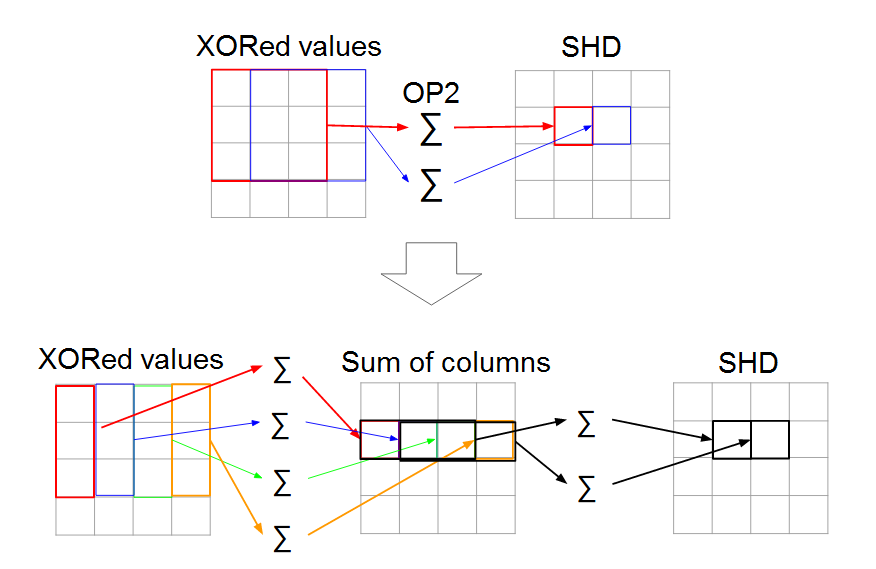
\includegraphics[width=.8\linewidth]{figures/parsumoptimization}
    \caption{Storage and reuse of partial SHD values.}
    \label{fig:parsumoptimization}
\end{figure}

The formula for SHD calculation is given in the Equation \ref{eqn:shd}. Consider the definition of OP2 provided in the Section \ref{s:optimizations:xoroptimization}. OP2 which is basically the sum of all elements within a window can be sequentially performed in many ways. One of the ways is first performing the sum of all columns and then performing the sum of results. It is noticeable that between positions (x,y) and (x+1,y), all but one column of the windows are the same. Hence, if the sum of columns are stored they can be reused across windows. For each element (x,y) the column vector of size same as the height of the window is summed up and stored. Then the required column vectors for each position (x,y) are summed up to provide the sum of elements of the window. This reuse of sum of column vectors reduces the number of calculations required for calculating the SHD at any position (x,y).  Optimization involving storage and reuse of partial SHD values is illustrated in the Figure \ref{fig:parsumoptimization}.

%%%%%%%%%%%%%%%%%%%%%%%%%%%%%%%%%%%%%
%%%%%%%%%%%%%%%%%%%%%%%%%%%%%%%%%%%%%
%%%%%%%%%%%%   SECTION   %%%%%%%%%%%%
%%%%%%%%%%%%%%%%%%%%%%%%%%%%%%%%%%%%%
%%%%%%%%%%%%%%%%%%%%%%%%%%%%%%%%%%%%%
\section{Optimized DM algorithm}
\label{sec:optdmalgo}

\begin{figure}
    \center
    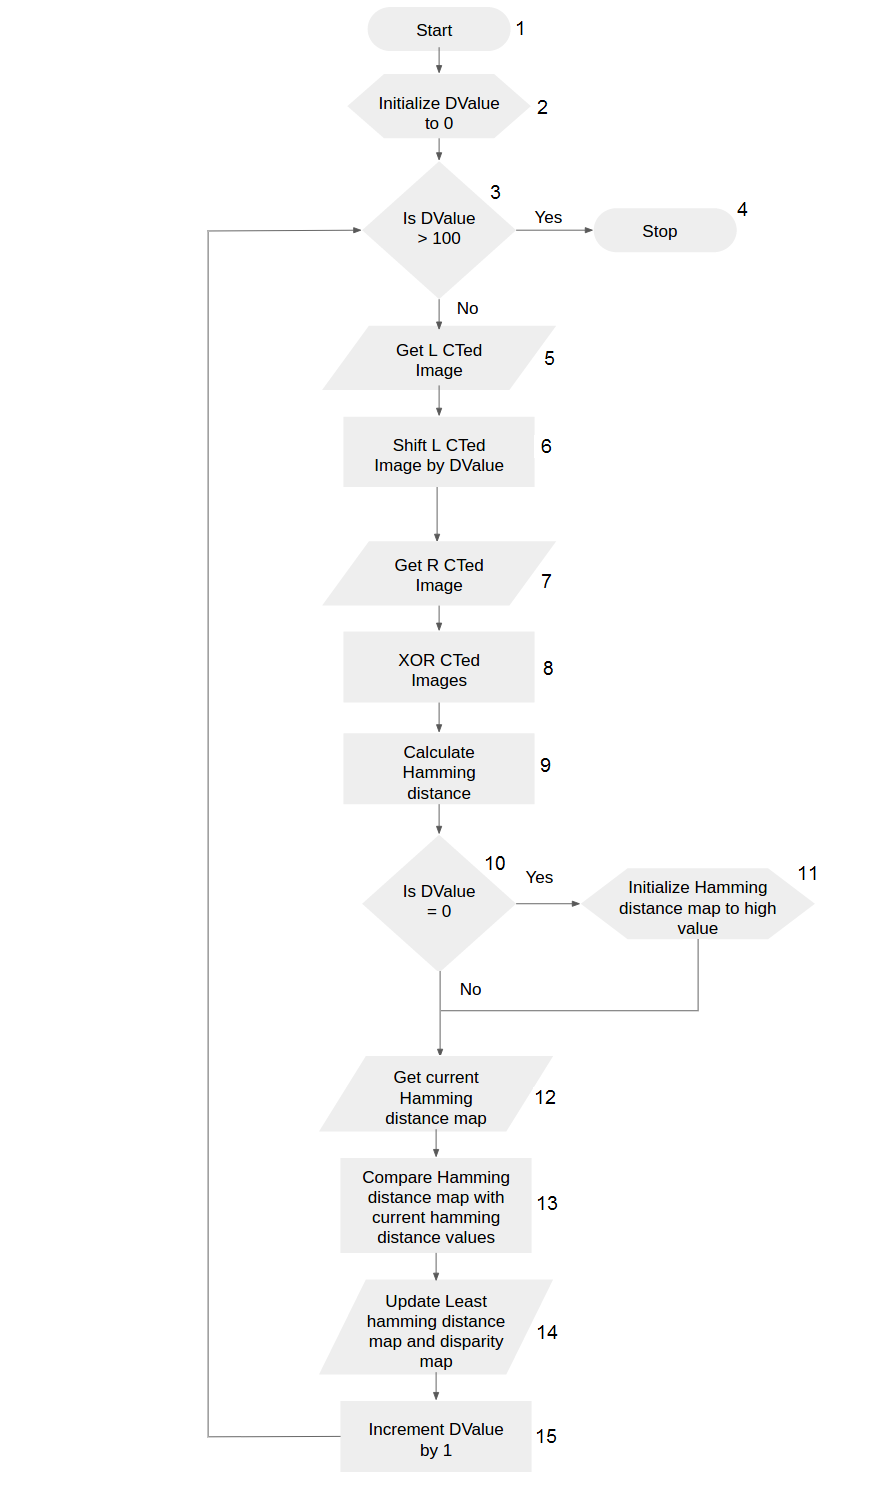
\includegraphics[width=.8\linewidth]{figures/shdalgorithm}
    \caption{Optimized version of DM algorithm.}
    \label{fig:shdalgorithm}
\end{figure}

The DM algorithm resulting after applying all the optimizations is shown in the Figure \ref{fig:shdalgorithm}. The flowchart shown is for the calculation of DM for a single frame after preprocessing is done. In the figure, the algorithm is shown to loop for 101 iterations, each iteration for a disparity value (DValue). DValue is initialized with 0 (2). The census transformed images are taken as inputs (5,7). The left image is shifted by the DValue (6). OP1 and OP2 from the Figure \ref{fig:xoroptimization} is done for the images (8,9). In the first iteration, a hamming distance map with very high values corresponding to each pixel is initialized. This map is compared with the hamming distances obtained from 9 for each pixel (13). The pixels of the hamming distance map are updated in case the new hamming distance from 9 is lower than the current value (14). The corresponding pixels in the DM are also updated with the current DValue (14). The DValue is incremented and the loop is iterated for the entire range of DValues (15,3). The updated DM once the loop is complete gives the required disparity values at each pixel.

%%%%%%%%%%%%%%%%%%%%%%%%%%%%%%%%%%%%%
%%%%%%%%%%%%%%%%%%%%%%%%%%%%%%%%%%%%%
%%%%%%%%%%%%   SECTION   %%%%%%%%%%%%
%%%%%%%%%%%%%%%%%%%%%%%%%%%%%%%%%%%%%
%%%%%%%%%%%%%%%%%%%%%%%%%%%%%%%%%%%%%
\section{Summary}
\label{sec:summary3}

The chapter discussed on the proposed algorithm and various optimizations done to it. The optimizations included software optimizations as shown in the Subsections \ref{s:optimizations:dsoptimization}, \ref{s:optimizations:multithreading}, \ref{s:optimizations:invariantcodemotion} and \ref{s:optimizations:simd}, and algorithm modifications as shown in the Subsections \ref{s:optimizations:xoroptimization} and \ref{s:optimizations:shdoptimization}. The resulting algorithm for DM creation was discussed. The effects of these optimizations and the effect of parameter change in the algorithm is discussed in the next chapter.
\chapter{Software Implementation Results}
\label{sec:aresults}

This chapter deals with the functional verification and execution time of the algorithm. The initial Matlab implementation is tried out with different pairs of stereo images and parameters to verify the functionality of the algorithm.  For this purpose BMPRE in DM in comparison with the ground truth is discussed. The outputs obtained are presented. Next, the run-time performance of various optimised versions of the C++ implementation across different hardware is discussed. Images from Tsukuba university \cite{Martull2012,Peris2012} and Middlebury university \cite{Scharstein2001,Scharstein2003} are used for the purpose of evaluation.
%

%%%%%%%%%%%%%%%%%%%%%%%%%%%%%%%%%%%%%
%%%%%%%%%%%%%%%%%%%%%%%%%%%%%%%%%%%%%
%%%%%%%%%%%%   SECTION   %%%%%%%%%%%%
%%%%%%%%%%%%%%%%%%%%%%%%%%%%%%%%%%%%%
%%%%%%%%%%%%%%%%%%%%%%%%%%%%%%%%%%%%%
\section{Parameters}
\label{sec:parameters}

The important parameters which determine the quality of the DM, and the run time of the selected algorithm are, \begin{itemize}
\item{The morphological opening window size (MW)}
\item{The census transform window size (CTW)}
\item{The range od disparity values (D range)}
\item{The SHD window size (SHDW)}
\end{itemize}

These parameters are varied among a range of values and the corresponding functionality of the algorithm is recorded. An optimal set of parameters from is chosen for the eGPU evaluation.

%%%%%%%%%%%%%%%%%%%%%%%%%%%%%%%%%%%%%
%%%%%%%%%%%%%%%%%%%%%%%%%%%%%%%%%%%%%
%%%%%%%%%%%%   SECTION   %%%%%%%%%%%%
%%%%%%%%%%%%%%%%%%%%%%%%%%%%%%%%%%%%%
%%%%%%%%%%%%%%%%%%%%%%%%%%%%%%%%%%%%%
\section{Functional verification results}
\label{sec:fverificationres}

The BMPRE method described in the Section \ref{s:stereovision:bmpre} is used for functional verification. In this section, the parameter values are varied and the corresponding BMPRE values are observed. The values giving the least BMPRE are chosen for the eGPU implementation.

%%%%%%%%%%%%%%%%%%%%%%%%%
%%%%%   SUB-SECTION   %%%
%%%%%%%%%%%%%%%%%%%%%%%%%
%%%%%%%%%%%%%%%%%%%%%%%%%
\subsection{Morphological opening window size (MW)}
\label{s:fverificationres:mw}

\begin{figure}
  \center
  \captionsetup{justification=centering}
  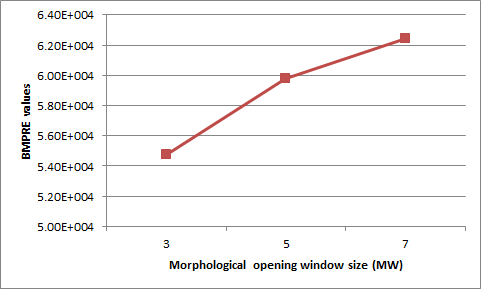
\includegraphics[width=.8\linewidth]{figures/BMPRE1}
  \caption{BMPRE values ($\delta$=2) across different MW values. Other parameters are kept constant with CTW=11, D range: 0-100, and SHDW=13}
  \label{fig:bmpre1}
\end{figure}


The Section \ref{s:algorithm:preprocessing} explains about the morphological opening operation. Different MW values are experimented while keeping the other parameters constant, and the BMPRE values are observed. In this experiment CTW is 11, D range ranges from 0 to 100, and SHDW is 13. The first frame of Tsukuba university image pair is chosen for evaluation. As indicated in the Section \ref{s:stereovision:bmpre} $\delta$ value is kept at 2. The results for MW values 3,5, and 7 are as shown in the Figure \ref{fig:bmpre1}. It can be seen that MW value of 3 yields the best results.

\subsection{Census transform window size (CTW) and disparity range (D range)}
\label{s:fverificationres:mw}

\begin{figure}
\captionsetup[subfigure]{justification=centering}
\begin{subfigure}{.5\textwidth}
  \centering
  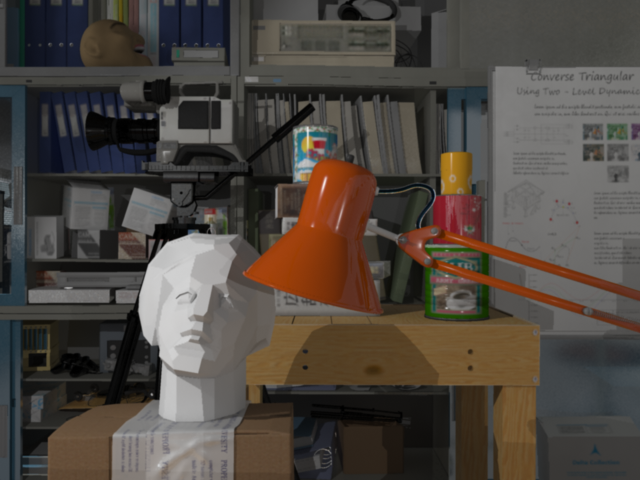
\includegraphics[width=.8\linewidth]{figures/frame_1_right}
  \caption{Original image (right)}
  \label{fig:sfig1}
\end{subfigure}
\begin{subfigure}{.5\textwidth}
  \centering
  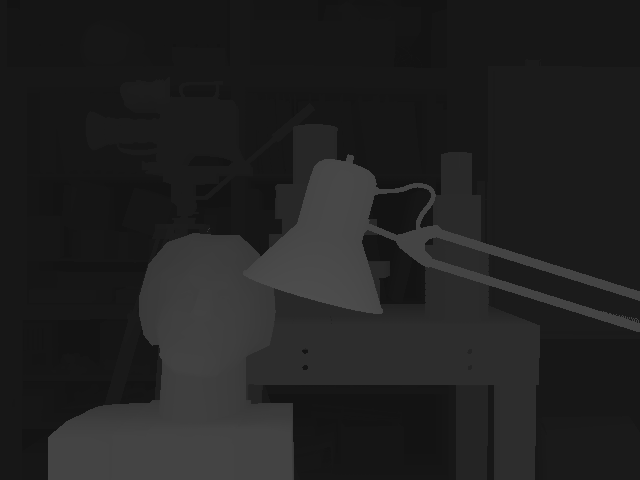
\includegraphics[width=.8\linewidth]{figures/frame_1}
  \caption{Ground truth}
  \label{fig:sfig2}
\end{subfigure}
\begin{subfigure}{.5\textwidth}
  \centering
  
\includegraphics[width=.8\linewidth]{figures/CT7D0-50}
  \caption{7x7 census transform window \\Disparity range 0 to 50}
  \label{fig:sfig3}
\end{subfigure}%
\begin{subfigure}{.5\textwidth}
  \centering
  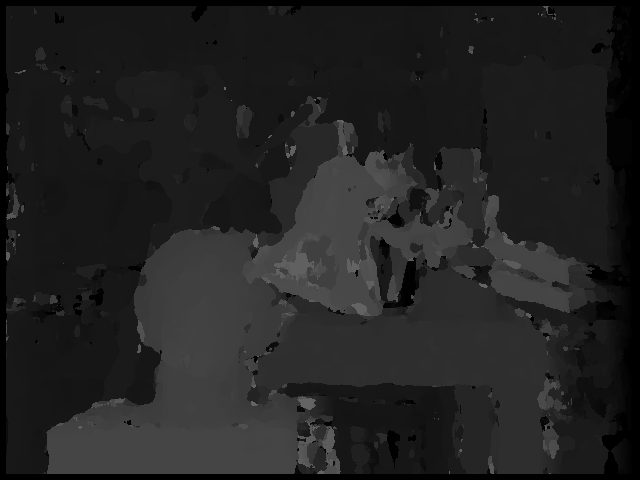
\includegraphics[width=.8\linewidth]{figures/CT7D0-100}
  \caption{7x7 census transform window \\Disparity range 0 to 100}
  \label{fig:sfig4}
\end{subfigure}
\begin{subfigure}{.5\textwidth}
  \centering
  
\includegraphics[width=.8\linewidth]{figures/CT9D0-50}
  \caption{9x9 census transform window \\Disparity range 0 to 50}
  \label{fig:sfig5}
\end{subfigure}%
\begin{subfigure}{.5\textwidth}
  \centering
  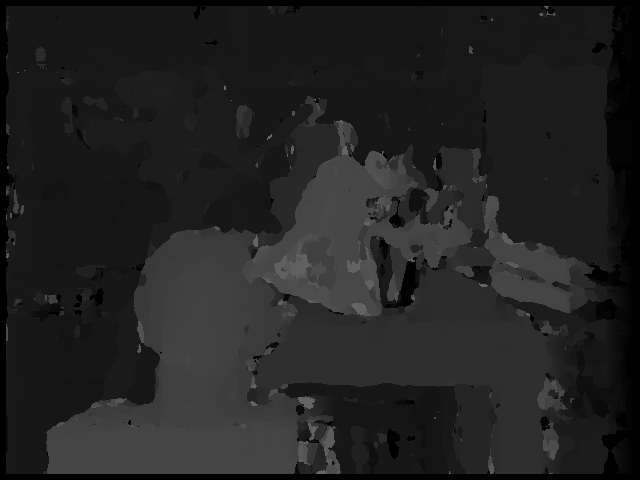
\includegraphics[width=.8\linewidth]{figures/CT9D0-100}
  \caption{9x9 census transform window \\Disparity range 0 to 100}
  \label{fig:sfig6}
\end{subfigure}
\begin{subfigure}{.5\textwidth}
  \centering
  
\includegraphics[width=.8\linewidth]{figures/CT11D0-50}
  \caption{11x11 census transform window \\Disparity range 0 to 50}
  \label{fig:sfig7}
\end{subfigure}%
\begin{subfigure}{.5\textwidth}
  \centering
  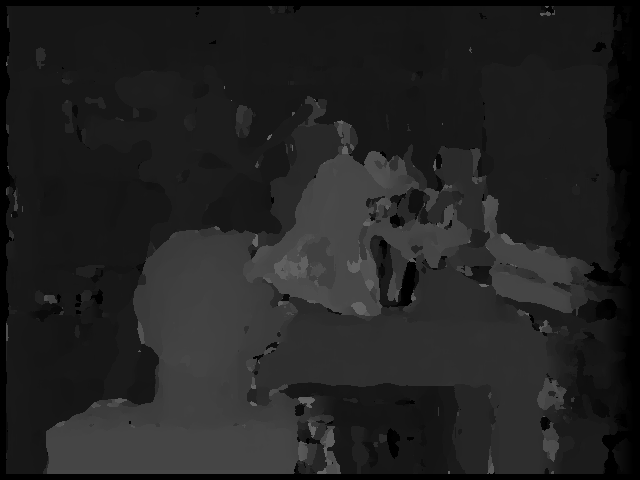
\includegraphics[width=.8\linewidth]{figures/CT11D0-100}
  \caption{11x11 census transform window \\Disparity range 0 to 100}
  \label{fig:sfig8}
\end{subfigure}
\caption{Disparity maps for Tsukuba image pair across different parameters}
\label{fig:dmappartsu}
\end{figure}


\begin{figure}
\captionsetup{justification=centering}
\captionsetup[subfigure]{justification=centering}
\begin{subfigure}{.5\textwidth}
  \centering
  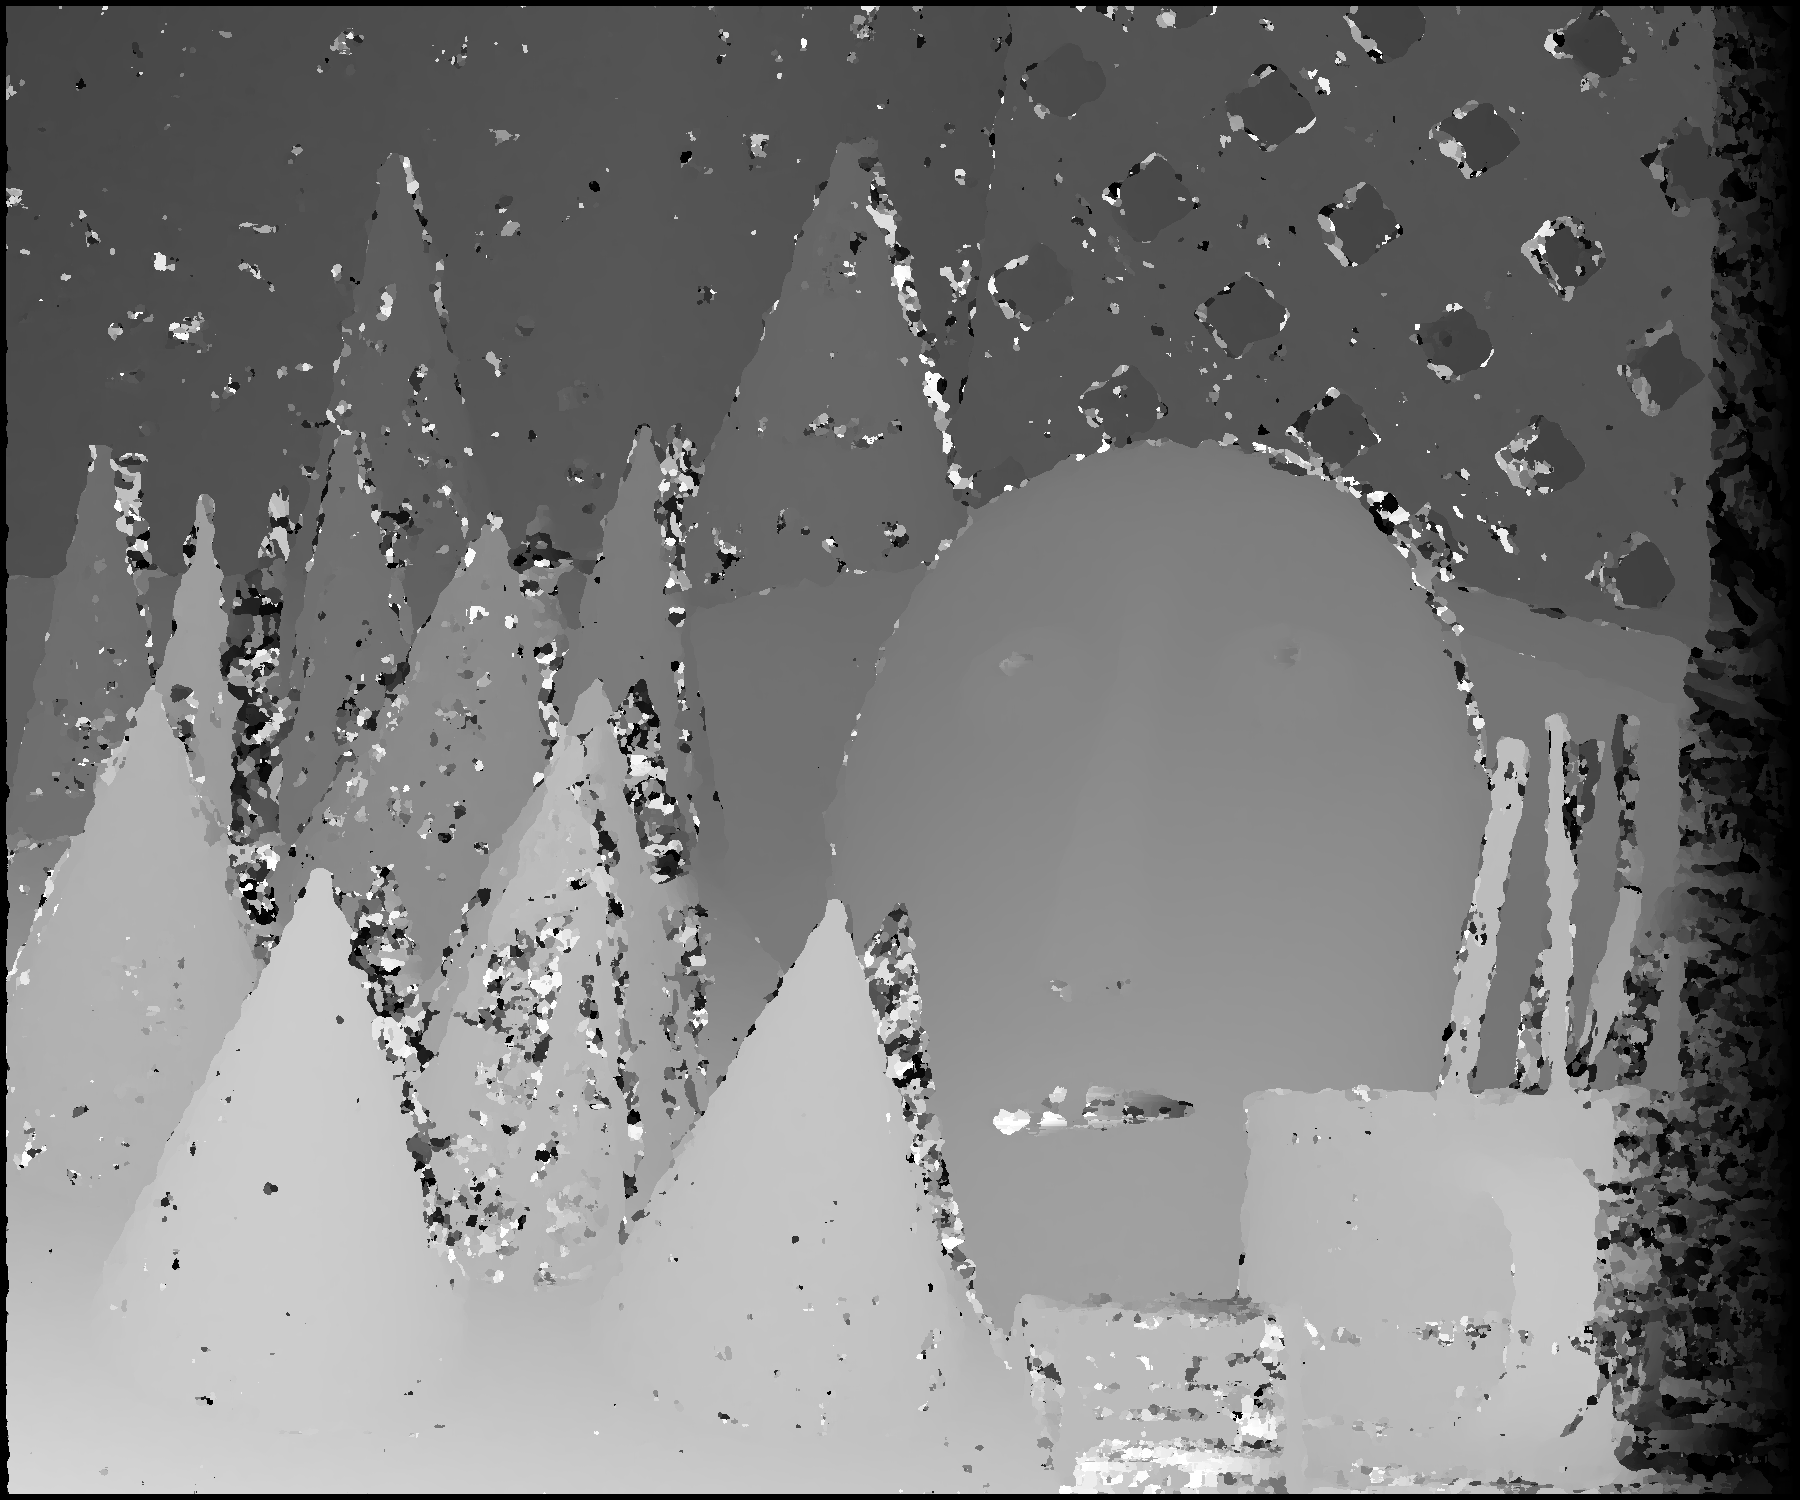
\includegraphics[width=.6\linewidth]{figures/ConeCT11D0-255}
  \caption{Disparity map}
  \label{fig:sfig1}
\end{subfigure}%
\begin{subfigure}{.5\textwidth}
  \centering
  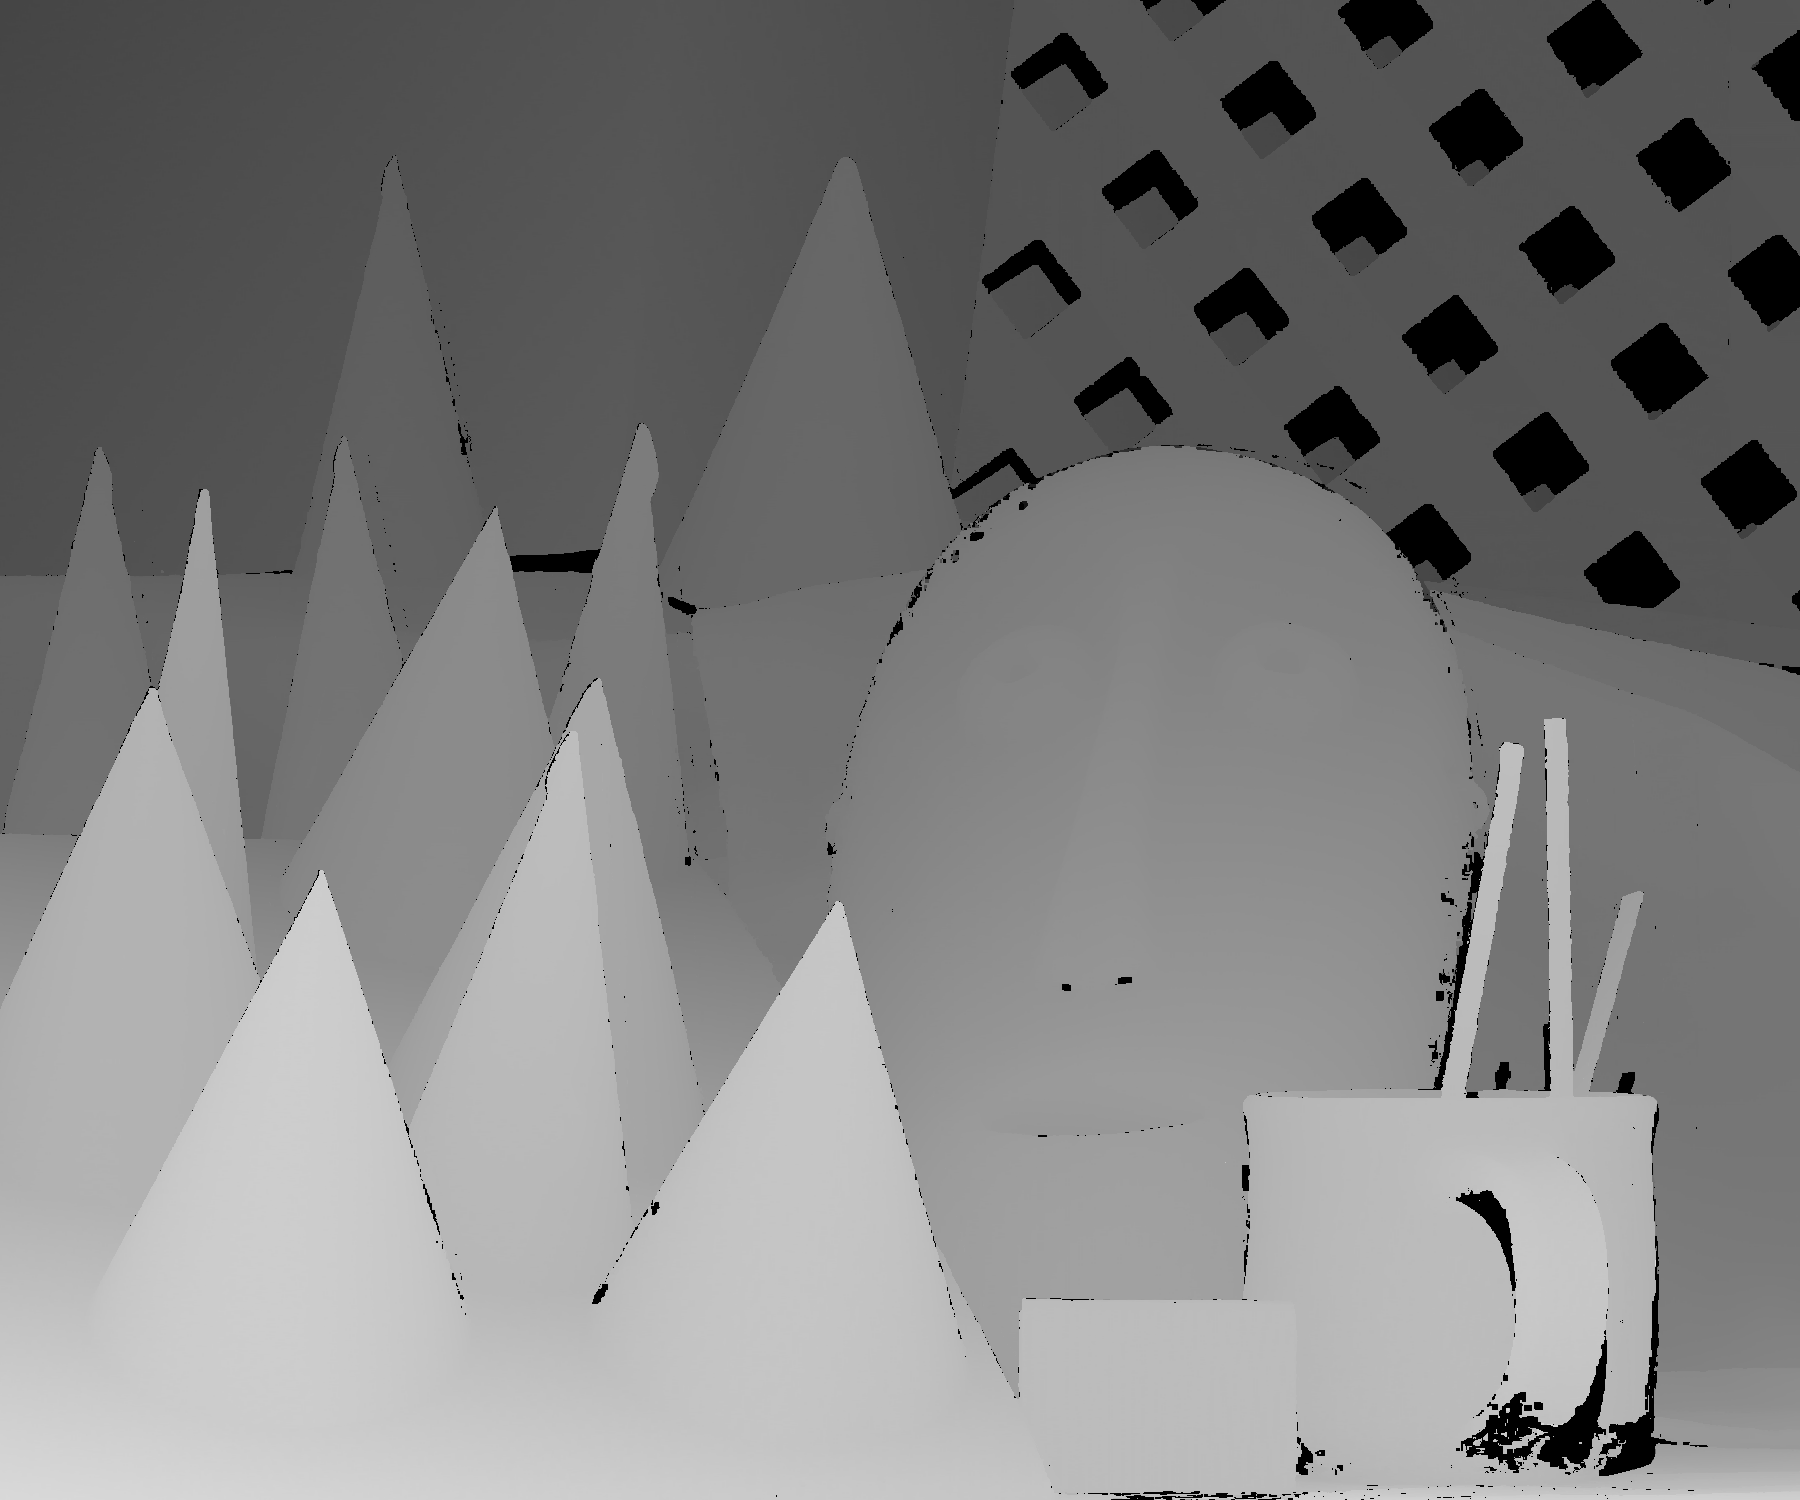
\includegraphics[width=.6\linewidth]{figures/ConeGT}
  \caption{Ground truth}
  \label{fig:sfig2}
\end{subfigure}
\caption{DM and ground truth for Cone(Middlebury) image pair with 11x11 census transform window and disparity range 0 to 255}
\label{fig:dmcone}
\end{figure}

% Please add the following required packages to your document preamble:
% \usepackage{booktabs}
\begin{table}[!htbp]
\centering
\begin{tabular}{@{}|c|c|c|c|c|c|@{}}
\toprule
\textbf{Image}        & \textbf{CT window size} & \textbf{Disp. Min.} & \textbf{Disp. Max} & \textbf{Resolution} & \textbf{BMPRE} \\ \midrule
Tsukuba frame 1       & 11                      & 0                   & 100                & 640x480             & 54800          \\ \midrule
Cone (Middlebury)     & 11                      & 0                   & 255                & 1800x1500           & 240000         \\ \midrule
Sawtooth (Middlebury) & 11                      & 0                   & 100                & 434x380             & 3161.3         \\ \bottomrule
\end{tabular}
\caption{BMPRE values ($\delta$=2) across images of different resolutions.}
\label{tab:bmpre}
\end{table}


The Figure \ref{fig:dmappartsu} shows the DM across different CTW and D range values for the Tsukuba university image pair along with the ground truth. The Table \ref{tab:bmpre} shows the BMPRE values (lower the better) across the images of different resolutions. The range of disparity values needs to be increased with resolution. This can be seen from the entry for Cone (Middlebury) in the table. Since that particular image pair is of high resolution, it requires greater number of disparity values for generating a detailed DM. The DM generated for the image pair can be seen in the Figure \ref{fig:dmcone}. It is also to be noted that BMPRE values probably increase with increase in resolution as more pixels are evaluated. This shows that the BMPRE values are not a global standard but depends on the resolution of the image.

\begin{figure}
  \center
  \captionsetup{justification=centering}
  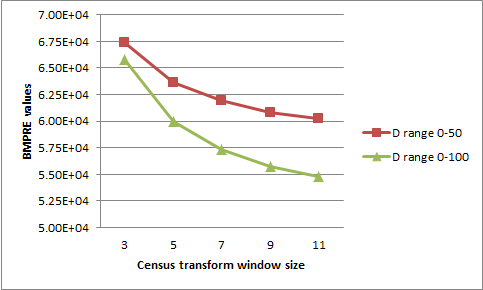
\includegraphics[width=.8\linewidth]{figures/BMPRE}
  \caption{BMPRE values across different CTW for different D ranges.}
  \label{fig:bmpre}
\end{figure}

 The effect of the window size and disparity range can be graphically seen in the Figure \ref{fig:bmpre}. This clearly shows the advantage of having larger census transform windows and greater range of disparity values. Census transform windows larger than 11 are not evaluated as it would require more than one data element(long integer) to store information for each pixel and might effectively nullify optimizations discussed in the Section \ref{sec:optimizations}.
 \\
From the observed results, the CTW value of 11 is chosen as it gives the best functional performance. D range of 0-100 is preferred as Tsukuba dataset is used, which is of resolution 640x480.

%%%%%%%%%%%%%%%%%%%%%%%%%
%%%%%   SUB-SECTION   %%%
%%%%%%%%%%%%%%%%%%%%%%%%%
%%%%%%%%%%%%%%%%%%%%%%%%%
\subsection{SHD window size (SHDW)}
\label{s:fverificationres:shdw}

\begin{figure}[!htbp]
  \center
  \captionsetup{justification=centering}
  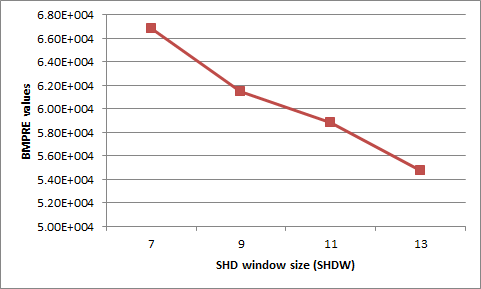
\includegraphics[width=.8\linewidth]{figures/BMPRE2}
  \caption{BMPRE values ($\delta$=2) across different SHDW values. Other parameters are kept constant with CTW=11, D range: 0-100, and MW=3}
  \label{fig:bmpre2}
\end{figure}

SHD calculation is a computational intensive calculation as it operates on a huge amount of data from the pre-processing stage. Census transformed (CTW=11) image yields 120 bits for every pixel in the image. SHDW plays an important role in determining the accuracy of DM. An experiment on the first frame from Tsukuba dataset across different SHDW values keeping the other parameters constant is performed. The results are as shown in the Figure \ref{fig:bmpre2}. It can be seen that SHDW value of 13 yields the best results for the tested values. Higher values of SHDW are not experimented owing to the computational intensity, which affects the execution time of the algorithm.

%%%%%%%%%%%%%%%%%%%%%%%%%%%%%%%%%%%%%
%%%%%%%%%%%%%%%%%%%%%%%%%%%%%%%%%%%%%
%%%%%%%%%%%%   SECTION   %%%%%%%%%%%%
%%%%%%%%%%%%%%%%%%%%%%%%%%%%%%%%%%%%%
%%%%%%%%%%%%%%%%%%%%%%%%%%%%%%%%%%%%%
\section{Algorithm run-time performance}

% Please add the following required packages to your document preamble:
% \usepackage{booktabs}
\begin{table}[!htbp]
\centering
\begin{tabular}{@{}|c|c|c|c|c|@{}}
\toprule
\textbf{Hardware}    & \textbf{RAM (GB)} & \textbf{Clock(GHz)} & \textbf{Cores} & \textbf{Threads} \\ \midrule
Intel Core i3-350M   & 3                 & 2.26                & 2              & 4                \\ \midrule
Intel Core i5-2500K  & 16                & 3.3                 & 4              & 4                \\ \midrule
Intel Core i7-5820K* & 32                & 3.3                 & 6              & 6                \\ \bottomrule
\end{tabular}
\captionsetup{justification=centering}
\caption{Hardware platform details. \\ *It is to be noted that Intel Corei7 was implemented using virtual machine.}
\label{tab:hwplat}
\end{table}

In this section, various optimized versions of algorithm discussed in the Section \ref{sec:optimizations} is evaluated for execution time across different hardware. The Table \ref{tab:hwplat} shows the details of the hardware platforms. Linux OS with the 3.13.0-85-generic kernel is used for implementation. A single frame-pair from the Tsukuba dataset is evaluated for the purpose. The versions of the algorithm are numbered as shown in Figure \ref{fig:algover} according to the optimizations involved. Optimizations which do not yield favourable results are avoided in the subsequent versions of the algorithm. The performance of algorithm across different hardware is as shown in the Figure \ref{fig:algort}.

\begin{figure}[!htbp]
    \center
    \captionsetup{justification=centering}
    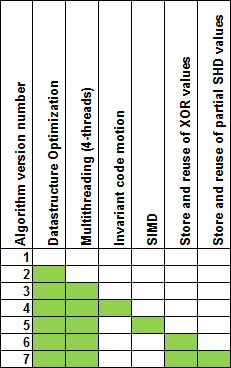
\includegraphics[width=.4\linewidth]{figures/AlgoVersions}
    \caption{Various versions of algorithm with the optimizations involved.}
    \label{fig:algover}
\end{figure}

\begin{figure}[!htbp]
    \center
    \captionsetup{justification=centering}
    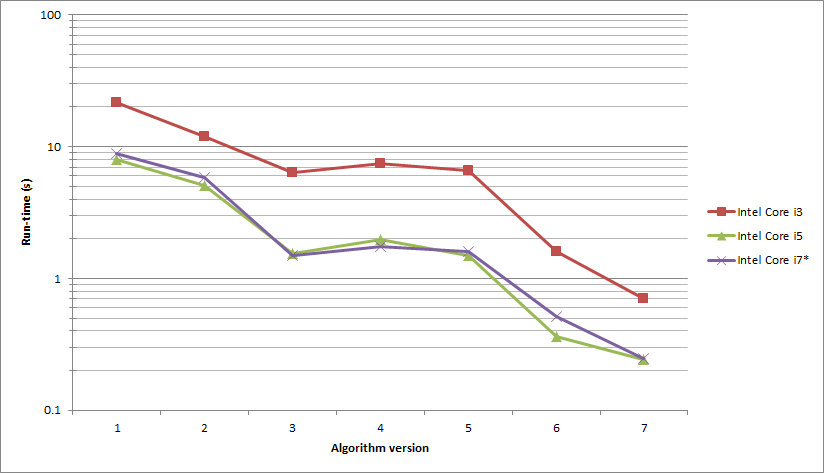
\includegraphics[width=\linewidth]{figures/Runtime}
    \caption{Runtime of various versions of algorithm across different hardware.\\ *It is to be noted that performance in Intel Corei7 was measured using virtual machine and hence might be relatively slower than actual performance}
    \label{fig:algort}
\end{figure}

The numbers shown in the Figure \ref{fig:algort} are from the C++ implementation of the algorithm in Linux with gcc 4.9.3 compiler. The values are obtained by running the algorithm 10 times and averaging the results in each case. The figure shows that algorithm performs better in Intel Corei5 and i7 compared to i3. This is due to the presence of more cores as indicated by the Table \ref{tab:hwplat} and hence better support for multi-threading. As indicated in the figure there does not seem to be much of speed up achieved in i7 implementation against i5, probably due to the fact that the i7 measurements were taken using a virtual machine, VMware.\\

From the figure, it can be seen that the optimizations Invariant code motion and  SIMD do not yeild favourable results. The reason for slower perfomance with Invariant code motion might probably be due to register spill as multiple threads are involved in executing the same code. SIMD optimization, as discussed in the Section \ref{s:optimizations:simd}, involves parallelizing the XOR calculation in SHD calculation. However, SHD calculation also involves calculating the bit count which cannot be sped-up using SIMD. This reduces the speed-up that can be achieved. Also the register spill discussed in the Section \ref{s:optimizations:invariantcodemotion} might come into play in this case as well due to multiple threads, thus resulting in a slow-down of the algorithm's performance.\\

The numbers indicated in the Figure \ref{fig:algort} are processing times, which exclude the time taken for the input of the image. An analysis done on the pre-processing time(Census transform), total processing time(SHD and pre-processing), and total program run-time reveals the following, for most optimized version of algorithm:
\begin{itemize}
\item{The inupt and output of images take about 15\% of the run time. This time would be replaced by the reading time from the camera and writing time to frame buffer in a real application. It is safe to assume that this time might not accumulate with every frame, but might result in a delay in output as dedicated hardware is involved.}
\item{The pre-processing takes about 48\% of the processing time. Most of the optimizations discussed in the Section \ref{sec:optimizations} involve optimizing the SHD part of the algorithm. Further research in optimizing the pre-processing part will effectively result in faster execution of the algorithm.}
\item{The most optimized version of the algorithm executes 31X, 32X and 35X faster than the unoptimized version in Intel core i3,i5 and i7 respectively.}
\item{The fastest execution time of the algorithm in any of the tested hardware is 0.2427636s for one frame. This is still 5 times slower than the execution time expected for real-time operation(20 fps). This suggests that further acceleration, is required for real-time operation.}
\end{itemize}

%%%%%%%%%%%%%%%%%%%%%%%%%%%%%%%%%%%%%
%%%%%%%%%%%%%%%%%%%%%%%%%%%%%%%%%%%%%
%%%%%%%%%%%%   SECTION   %%%%%%%%%%%%
%%%%%%%%%%%%%%%%%%%%%%%%%%%%%%%%%%%%%
%%%%%%%%%%%%%%%%%%%%%%%%%%%%%%%%%%%%%
\section{Summary}
This chapter discussed on the method used for functional verification. The important parameters of the algorithm were discussed. The functional performance of the algorithm across different parameters was persented. MW of 3, CTW of 11, D range of 0-100 and SHDW of 13 were chosen for implementation in Nema. Subsequently, the execution time of the algorithm across various hardware was presented and valid optimizations were chosen. Valid optimizations provide 31X to 35X speed up based on the hardware implemented. Further observations were recorded.
\chapter{Implementation and evaluation of eGPU}
\label{chap:implementation}

The Section \ref{s:gpusw:nema} discussed on the software implementation in Nema GPU. This chapter discusses the implementation of the algorithm chosen and its results in functionality and run-time performance in the eGPU. The version 7 of the algorithm indicated in the Figure \ref{fig:algover} is used for evaluation purpose. For the purpose of comparison, the algorithm is also implemented in the hardware without the use of eGPU. This would help isolate the performance with and without eGPU. Observations are recorded.
%

%%%%%%%%%%%%%%%%%%%%%%%%%%%%%%%%%%%%%
%%%%%%%%%%%%%%%%%%%%%%%%%%%%%%%%%%%%%
%%%%%%%%%%%%   SECTION   %%%%%%%%%%%%
%%%%%%%%%%%%%%%%%%%%%%%%%%%%%%%%%%%%%
%%%%%%%%%%%%%%%%%%%%%%%%%%%%%%%%%%%%%
\section{Choice of kernels}
\label{sec:kernelchoice}

\begin{figure}
    \center
    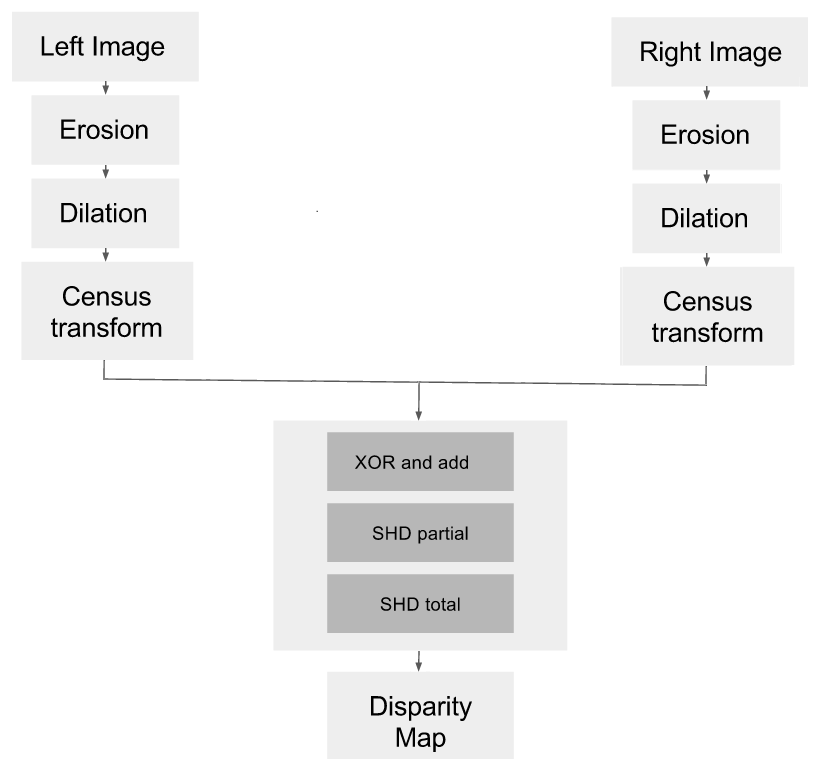
\includegraphics[width=.7\linewidth]{figures/Algorithm}
    \caption{Block diagram of algorithm implemented.}
    \label{fig:algorithm}
\end{figure}

The Figure \ref{fig:algorithm} shows the block diagram of the algorithm implemented. Here all the blocks can take advantage of eGPU parallelization as each of them perform the same operation across all the pixels. Hence, a kernel is written for each of the steps. For the purpose of SHD calculation, three kernels are required. This is due to lack of synchronization facilities between threads as discussed in the Section \ref{s:gpusw:nkernels}. For example, the partial SHD calculation part needs to be performed only after the XOR add step is completed for all the pixels. In Nema, it is not possible to implement both of them in a single kernel as there is no way of determining within a thread if all other threads have completed till certain step of the algorithm. This is a disadvantage as SHD involves loop operation with disparity value as a parameter as explained in the Section \ref{sec:optdmalgo}. This means three kernels need to be loaded for each iteration for XOR add, SHD partial and SHD total respectively. The function was experimented by using a single kernel and using conditional statements to decide on the thread functionality. However, this resulted in a slower performance probably due to incorrect branch predictions involved. Hence, a kernel for morphological erosion, morphological dialation, census transform, XOR addition, partial SHD calculation and total SHD calculation were created. This results in multiple kernels getting loaded for each iteration of the DM algorithm discussed in \ref{sec:optdmalgo}.
%

%%%%%%%%%%%%%%%%%%%%%%%%%%%%%%%%%%%%%
%%%%%%%%%%%%%%%%%%%%%%%%%%%%%%%%%%%%%
%%%%%%%%%%%%   SECTION   %%%%%%%%%%%%
%%%%%%%%%%%%%%%%%%%%%%%%%%%%%%%%%%%%%
%%%%%%%%%%%%%%%%%%%%%%%%%%%%%%%%%%%%%
\section{Functional Performance}
\label{sec:fperformance}

% Please add the following required packages to your document preamble:
% \usepackage{booktabs}
\begin{table}[!htbp]
\centering
\begin{tabular}{@{}|c|c|c|@{}}
\toprule
\textbf{Image}  & \textbf{BMPRE Intel Corei3} & \textbf{BMPRE zc706+Nema} \\ \midrule
Tsukuba frame 1 & 54762                       & 54499                     \\ \bottomrule
\end{tabular}
\caption{BMPRE across different hardware including Nema eGPU}
\label{tab:bmprenema}
\end{table}

\begin{figure}
    \center
    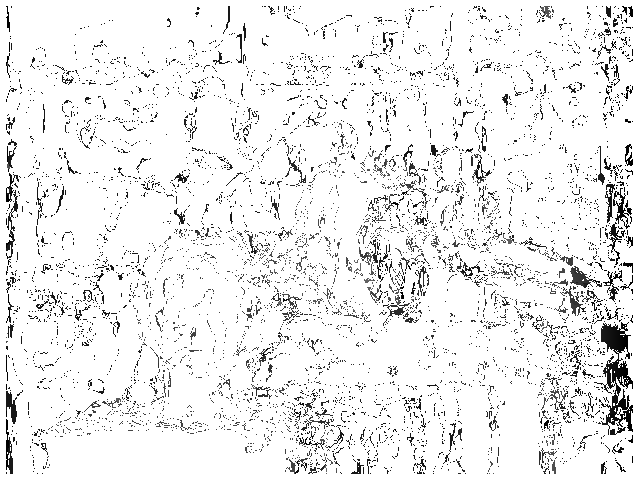
\includegraphics[width=.7\linewidth]{figures/diffpixeGPU}
    \caption{Pixels in eGPU disparity map that are different from Intel Core i3 disparity map.}
    \label{fig:diffpixegpu}
\end{figure}
As discussed in the beginning of this chapter, the algorithm is run with and without the eGPU for the purpose of performance comparison. BMPRE method discussed in the Section \ref{s:stereovision:bmpre} is used for functional evaluation. Ideally, same functional performance as observed in the software implementation is expected while using hardware. The first frame of Tsukuba dataset is used for the functional verification purpose. The Table \ref{tab:bmprenema} shows the BMPRE values in Intel Corei3, zc706 evaluation board with the Nema eGPU. It can be seen that there is a marginal difference in the values across hardwares, with the eGPU performing better. In order to understand the reason behind this, the pixels which are different from the Intel Corei3 result are looked into. The Figure \ref{fig:diffpixegpu} shows the pixels which are different in eGPU implementation from the Intel Core i3 implementation. There is not a particular pattern in the location of these pixels. Hence, the idea of these pixels arising due to synchronization between threads in Intel version of the program can be rejected. Further analysis needs to be done with more image sets to narrow down the reason for the difference.

%%%%%%%%%%%%%%%%%%%%%%%%%%%%%%%%%%%%%
%%%%%%%%%%%%%%%%%%%%%%%%%%%%%%%%%%%%%
%%%%%%%%%%%%   SECTION   %%%%%%%%%%%%
%%%%%%%%%%%%%%%%%%%%%%%%%%%%%%%%%%%%%
%%%%%%%%%%%%%%%%%%%%%%%%%%%%%%%%%%%%%
\section{Execution time}
\label{sec:rtperformance}

% Please add the following required packages to your document preamble:
% \usepackage{booktabs}
\begin{table}[!htbp]
\centering
\begin{tabular}{@{}|l|l|l|l|@{}}
\toprule
\multicolumn{1}{|c|}{\textbf{Hardware}} & \multicolumn{1}{c|}{\textbf{Work time (eGPU)(s)}} & \multicolumn{1}{c|}{\textbf{Work time (host)(s)}} & \textbf{Program execution time(s)} \\ \midrule
Intel core i3                           &                                                        &                                                      & 0.7010273                    \\ \midrule
zc706                                   &                                                        &                                                      & 5.95241                      \\ \midrule
zc706+Nema                              & 32.665                                                 & 39.3129                                              & 40.9769                      \\ \bottomrule
\end{tabular}
\caption{Execution time of algorithm in Nema in comparison with other hardware. The time eGPU is active as measured by the eGPU itself (Work time (eGPU)) and the host processor (Work time (host)) are indicated. Program execution time indicates the total execution time including the image I/O.}
\label{tab:nemart}
\end{table}

In order to gauge the execution time, the algorithm is run in zc706 hardware with and without the Nema GPU. Again frame 1 from the Tsukuba dataset is used for the evaluation. The Table \ref{tab:nemart} shows the difference in execution time of the algorithm across different hardware. The table shows two entries for work time of the Nema eGPU. Worktime (host) is measured by the program running on the host processor. It is the difference in time between command list is flushed, and an interrupt indicating Nema operation is complete is raised. Work time (eGPU) is the time Nema cores are active as measured by the internal hardware of eGPU. It can be seen that host indicates a higher time compared to the one indicated by the GPU. This probably means that Nema cores are idle for some time during the execution of threads.

\begin{figure}[!htbp]
\captionsetup{justification=centering}
\captionsetup[subfigure]{justification=centering}
\begin{subfigure}{.5\textwidth}
  \centering
  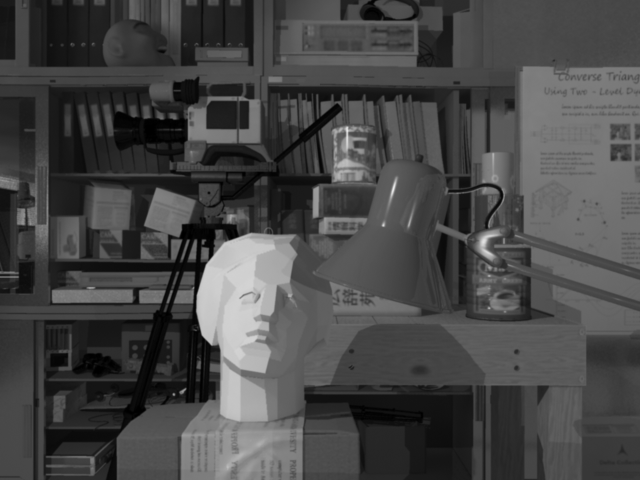
\includegraphics[width=.8\linewidth]{figures/frame_1_monochrome}
  \caption{Monochrome image.}
  \label{fig:sfig1}
\end{subfigure}%
\begin{subfigure}{.5\textwidth}
  \centering
  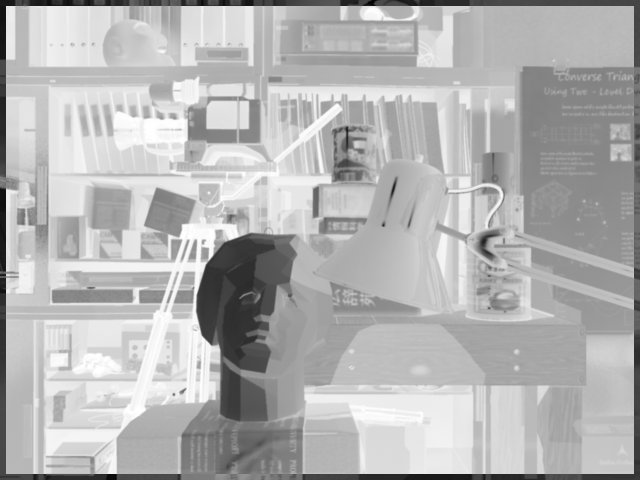
\includegraphics[width=.8\linewidth]{figures/negated}
  \caption{Negated image.}
  \label{fig:sfig2}
\end{subfigure}
\caption{Negation of left camera monochrome image, frame 1, Tsukuba dataset.}
\label{fig:negation}
\end{figure}


The algorithm is seen to run slower with the Nema GPU compared to the case without it. There could be possibly few factors behind this. 
\begin{itemize}
\item{Nema runs at a slower speed(83MHz) compared to the host processor(800MHz). Silicon implementation of Nema will result in a faster performance.}
\item{From the Section \ref{sec:kernelchoice} it can be seen that there are three kernels loaded for each iteration of the program. It might be possible that the kernel loading time is much higher than the actual execution time. However Work time (eGPU) from the Table \ref{tab:nemart} suggests that execution time is higher. As a sanity check a simpler program with a single kernel, loaded only once is evaluated at runtime. The program performs negation of pixels as shown in the Figure \ref{fig:negation}.The results are as shown in the first row of the Table \ref{tab:nemartneg}. This confirms that loading of kernels is not the prime factor influencing the slower run-time.}
\item{The slowdown could be a result of poor hardware thread management. Since Nema has only 4 cores with 16 threads each, only 64 threads can run at a time. A software thread management experiment was done by programatically deploying 64 threads at a time, and waiting for them to complete before deploying the next 64 threads and so on. This was done for the negate program to find out if the eGPU's hardware thread management was slowing the system down. However, this turned out not to be true as shown in the second row of the Table \ref{tab:nemartneg}. Note that the Nema working time as measured by the eGPU itself is shown as zero as each set of threads complete within a span of a ms, thus being too fast to measure.}
\item{Nema has a common data cache of 1MB for all the four cores. Each core runs independently of the others, so each core most likely executes a different part of the kernel. Since cores can operate on different data points along the image, there might be data conflict between the cores leading to high miss rates. This cannot be confirmed as currently Nema does not keep track of cache statistics.}

\end{itemize}

% Please add the following required packages to your document preamble:
% \usepackage{booktabs}
\begin{table}[!htbp]
\centering
\begin{tabular}{@{}|c|c|c|c|@{}}
\toprule
\textbf{Program}                  & \textbf{Work time (eGPU)(s)} & \textbf{Work time (host)(s)} & \textbf{Program run time(s)} \\ \midrule
Negate & 0.016                             & 0.0351441                       & 0.913559                     \\ \midrule
Negate (software thread management) & 0                                 & 77.3031                         & 78.1798                      \\ \bottomrule
\end{tabular}
\caption{Nema execution time results for the Negate program with and without software thread management.}
\label{tab:nemartneg}
\end{table}
\chapter{Conclusion}
\label{chap:conclusion}


%%%%%%%%%%%%%%%%%%%%%%%%%%%%%%%%%%%%%
%%%%%%%%%%%%%%%%%%%%%%%%%%%%%%%%%%%%%
%%%%%%%%%%%%   SECTION   %%%%%%%%%%%%
%%%%%%%%%%%%%%%%%%%%%%%%%%%%%%%%%%%%%
%%%%%%%%%%%%%%%%%%%%%%%%%%%%%%%%%%%%%
\section{Summary}

The aim of the thesis was to study the effects of parameter variations and software optimizations of a Stereo vision algorithm and further evaluate the Nema eGPU using the algorithm. The work began with the explanation of the importance of Stereo vision and eGPU. The problems to be tackeled were discussed and phrased. Requirements of an algorithm to be studied were identified. The problems arising due to the nature of the application and the hardware were listed and explanation was given how they were tackled. Different parts of algorithm were identified and choice of methods in each part of algorithm was explained and justified. A list of optimizations to improve the execution time of the algorithm were proposed and a justification was presented on why the optimizations could work. A series of experiments varying the parameters of the chosen algorithm were performed. In each case the functional performance of the algorithm was measured using BMPRE method proposed by Cabezas et al. \cite{Cabezas2012}. Set of parameters yielding the best functional performance were chosen. The execution time for each version of algorithm with different optimizations proposed were presented. The cases for which speed up was not achieved were discussed with possible arguments. The algorithm was implemented in Nema eGPU. The functional performance and the execution time of the algorithm were observed. Possible reasons for the observations are discussed and further experiments were performed where possible to refine the observations.


%


%%%%%%%%%%%%%%%%%%%%%%%%%%%%%%%%%%%%%
%%%%%%%%%%%%%%%%%%%%%%%%%%%%%%%%%%%%%
%%%%%%%%%%%%   SECTION   %%%%%%%%%%%%
%%%%%%%%%%%%%%%%%%%%%%%%%%%%%%%%%%%%%
%%%%%%%%%%%%%%%%%%%%%%%%%%%%%%%%%%%%%
\section{Conclusion}

\begin{itemize}
\item{SHD algorithm along with preprocessing including morphological opening and census transform were found to be suitable for the eGPU evaluation.}
\item{The parameters MW = 3, CTW = 11, D value: 0-100, and SHDW = 13 were found to provide the best functional results for the chosen algorithm.}
\item{Optimization of the algorithm yielded in 31X, 32X and 35X improvement in execution time in Intel core i3,i5, and i7 respectively.}
\item{After optimizing the algorithm in various aspects it was found that it fell short of real-time performance in hardwares including Intel Core i3, i5 and i7.}
\item{For the chosen dataset, functionally eGPU performs marginally better than Intel Core i3 processor. Further analysis with more dataset needs to be done to reason out the increase in functional performance of eGPU.}
\item{The eGPU performs considerably slower than the implementation without the eGPU. The slow down is not dependent on the kernel choice or poor thread management.}
\item{The slow down of the eGPU might be attributed to slower clocking of the GPU and high miss rate of data. Further research needs to be done in this direction for more accurate results.}
\end{itemize}

%

%%%%%%%%%%%%%%%%%%%%%%%%%%%%%%%%%%%%%
%%%%%%%%%%%%%%%%%%%%%%%%%%%%%%%%%%%%%
%%%%%%%%%%%%   SECTION   %%%%%%%%%%%%
%%%%%%%%%%%%%%%%%%%%%%%%%%%%%%%%%%%%%
%%%%%%%%%%%%%%%%%%%%%%%%%%%%%%%%%%%%%
\section{Suggestions for future work}
\begin{itemize}
	\item{Further optimization can be done on the algorithm to increase the performace speed. Two possible optimizations can be:}
	\begin{itemize}
		\item{SHD can be further optimized by subtracting the first row and adding the next row to get the SHD value for the next pixel}
		\item{The each bit in census transform is not completely independent. Bits of census transformed pixels present in the census transformed window might be reused to boost performance.}
	\end{itemize}
	\item{Further analysis needs to be done to identify the change in functional performance between the hardware discussed ans eGPU}
	\item{The algorithm can be deployed in the silicon implementation of the eGPU and performance analysed.}
	\item{The cache activities can be tracked to further confirm the reason behind the slow down of eGPU performance.}
\end{itemize}

%BIBLIOGRAPHY
\addcontentsline{toc}{chapter}{Bibliography}
\bibliographystyle{IEEEtran}
\fancyhead[RE]{\normalfont Bibliography}
\fancyhead[LO]{\normalfont Bibliography}
\bibliography{bibliography/References}


APPENDIX
\appendix
\chapter{Appendix}
\label{chap:appendix}

%%%%%%%%%%%%%%%%%%%%%%%%%%%%%%%%%%%%%
%%%%%%%%%%%%%%%%%%%%%%%%%%%%%%%%%%%%%
%%%%%%%%%%%%   SECTION   %%%%%%%%%%%%
%%%%%%%%%%%%%%%%%%%%%%%%%%%%%%%%%%%%%
\section{Nema kernel for morphological erosion}
\label{s:kerero}

\lstset {language=C++}
\begin{lstlisting}

#include "macros.h"

extern "C" 
{

  #define USE_PIXOUT

  __attribute__((naked)) void shd()
  {
    unsigned char *input, *output, min;
    int row, column;

    read_reg(row, "v128.x");//Read constant register value to get the total number of rows
    read_reg(column, "v128.y");//Read constant register value to get the total number of columns
  
    ui_vec4 coords;
    read_coords(coords);//Read coordinates of the thread
    
    read_reg(input, "v0.w"); /// Read value from interpolator 0
    read_reg(output, "v0.z"); /// Read value from interpolator 1
  
    if(coords.x>1 && coords.x<(column-1) &&coords.y>1 && coords.y<(row-1))
    {
      min = *input;
      for (int k = -1; k <= 1; k++)
      {
        for (int l = -1; l <= 1; l++)
        {
          if (*(input+ k*column+ l) < min)
          {
            min = *(input + k*column + l);
          }
        }
      }
      *output = min;
    }
  }

} // extern "C"

\end{lstlisting}

\hfill \break

%%%%%%%%%%%%%%%%%%%%%%%%%%%%%%%%%%%%%
%%%%%%%%%%%%%%%%%%%%%%%%%%%%%%%%%%%%%
%%%%%%%%%%%%   SECTION   %%%%%%%%%%%%
%%%%%%%%%%%%%%%%%%%%%%%%%%%%%%%%%%%%%
%%%%%%%%%%%%%%%%%%%%%%%%%%%%%%%%%%%%%
\section{Section of Nema host program invoking the eGPU}
\label{s:hostero}

\lstset {language=C++}
\begin{lstlisting}

...
void Nema::erode(unsigned char* input,unsigned char *output, int row, int column)
{
  int width, height;

  void *bin = nema_load_binary("kernels/erode.bin"); /// Load binary
  assert(bin);

  tsi_cmdl_add_cmd(NEMA_FRAG_PTR, ::nema_virt_to_phys((uint32_t)bin));/// Converting virtual address to physical address

  /// Now that the video dimensions are known reprogram rasterizer and the interpolators
  width  = column;
  height = row;

    /// Everything drawn outside this viewport is clipped out
  tsi_cmdl_add_cmd(NEMA_TARGET_RESOL,  (height << 16) | width);

    /// Set up rasterizer dimensions
    /// The rasterizer will generate ( width - 1 ) x ( height - 1 ) threads
  tsi_cmdl_add_cmd(NEMA_VERTEX1_X, width - 1);
  tsi_cmdl_add_cmd(NEMA_VERTEX1_Y, height - 1);

  tsi_cmdl_add_cmd(NEMA_VAR0_V1_0, width);   /// Interpolator 0 stride
  tsi_cmdl_add_cmd(NEMA_VAR0_V2_0, 1);       /// Interpolator 0 step

  tsi_cmdl_add_cmd(NEMA_VAR0_V1_1, width);   /// Interpolator 1 stride
  tsi_cmdl_add_cmd(NEMA_VAR0_V2_1, 1);       /// Interpolator 1 step

  /// Setup Interpolators
  tsi_cmdl_add_cmd(NEMA_VAR0_V0_0, (uint32_t)nema_virt_to_phys((uint32_t)input)); /// Interpolator 0 start
  tsi_cmdl_add_cmd(NEMA_VAR0_V0_1, (uint32_t)nema_virt_to_phys((uint32_t)output)); /// Interpolator 1 start

  ///Store the image dimensions as constants
  Nema_setconst(0, 0, row);
  Nema_setconst(0, 1, column);

  /// Start the rasterizer
  tsi_cmdl_add_cmd(HOLD_DMA | NEMA_RAST_CMD, 0x02);


  nema_cmdl_flush_caches();
  tsi_cmdl_emit_commands(0);
}
...
\end{lstlisting}

\backmatter
%\include{cv}

\end{document}
